% 基于区块链的物联网时序数据高效存储技术研究

\chapter{绪论}
\section{研究背景及意义}
近年来,物联网(Internet of Things,IoT)发展迅速,促进了农业、制造业、医疗保健、零售业和公用事业等众多应用的发展。
根据Gartner的分析~\cite{hung2017leading},目前已部署的数十亿物联网设备将产生泽字节(ZettaBytes, ZB)的数据。
根据IoT的发展趋势可以预见,未来将有越来越多的数据集成到网络中。
对于如此大规模的数据,如果使用集中式服务器(例如AWS IoT、阿里云等)来管理,可能会遇到单点故障等问题~\cite{gill2011understanding}。
尽管分布式数据库可以避免单点故障,但由于其数据安全性和不可篡改性较弱,在需要高度透明的场景下,它们很容易受到数据篡改攻击~\cite{chen2022blockchain}。

以可追溯性和不变性为特征的区块链,可以解决集中式存储的单点故障问题和分布式数据库的恶意篡改问题。
它将数据存储在去中心化的账本中,使用共识协议来解决每个节点之间可能发生的冲突。
这种方式增强了安全性,提高了透明度,降低了成本,且支持平等节点间的协作。
然而,基于区块链的存储系统由于其较低的交易速度和较高的计算要求~\cite{dorri2017towards},仅广泛应用于价值巨大但密度很低的领域,如金融服务、供应链管理等。

目前,有许多研究人员致力于提高基于区块链的存储系统的性能。
根据数据的存储位置,这些工作可以分为两类,即链上存储和链下存储。

对于链上存储,数据作为存储在区块链上的交易记录的一部分。
用户通过区块链中的索引,即默克尔树来获取这些数据。
现有工作通过提供用户友好的查询语言~\cite{zhu2019sebdb,xu2019vchain,wang2022vchain+}提高了系统可用性,并通过改进索引方案~\cite{li2023lvmt,zhang2024cole}、区块链存储分片~\cite{zamani2018rapidchain,hong2023gridb,el2019blockchaindb}等方式提高系统吞吐量。
然而,在链上存储物联网数据的开销非常高。
对于大量快速生成的物联网数据,将其连续存储在区块链上需要实现共识和账本复制的过程,这可能会导致巨大的存储压力和通信开销。
因此,物联网数据存储的一种更实用的方法是使用链下存储方案。

对于链下存储,数据存储在区块链之外的存储节点,区块链只存储必要的元数据或对数据的引用,如哈希或加密指针。
链下存储提供了比链上解决方案更大的可扩展性和更低的成本,因此业界和学术界对链下存储非常有兴趣,例如Storj~\cite{storj2018storj}、BigchainDB~\cite{mcconaghy2016bigchaindb}、Sia~\cite{sia}等。
然而,现有的工作大多是为存储大文件而设计的。
对于单位粒度较小的物联网数据,考虑到物联网的海量大小,在区块链中存储每个数据项的哈希值将产生难以接受的开销。
此外,物联网应用场景通常需要存储系统支持高效查询(例如聚合查询),而现有的基于文件的存储系统不支持这一点。

本文基于链下存储的方案,提出了一种面向物联网的区块链存储系统,并基于该系统进行了一系列广泛的测量。
针对测量中发现的性能瓶颈,本文提出了TimeChain,一个基于区块链的物联网时序数据高效可信存储系统。
实验结果表明,TimeChain相比现有的基于区块链的存储系统有显著的性能提升,对于实现物联网数据的可信高效存储具有一定的理论和实践价值。

\section{论文主要工作}
为了对海量物联网数据进行可信、高效的存储,受链下存储方案的启发,本文提出了一种基于区块链的物联网时序数据基本存储方案。
该方案将数据分成多个批次,仅将每批数据的哈希值存储在链上,并将完整的原始数据保存在链外。
这种批处理存储方法大大减少了数据开销。
本文对该方案的性能进行了测量。
结果表明,与每个数据单独存储相比,将数据批量存储的存储延迟平均减少了37.4倍。
这种存储性能的显著提升使得区块链支持物联网数据存储成为可能。

然而,不可否认的是,这样的批处理方案会影响查询性能。
具体来说,当用户执行范围查询时,低效的聚合方法会导致在多个传输节点上获取数据,从而导致额外的传输延迟。
如果在节点选择过程中选择了不合适的节点,则可能会导致更高的数据传输延迟或较差的数据存储服务质量。
此外,由于区块链上只存储了批处理单元的哈希值,因此存储系统必须传输额外的信息(例如默克尔树的哈希路径),以支持数据拥有者执行数据完整性验证。
这进一步增加了查询开销。

针对测量中发现性能瓶颈的三个根本原因,本文提出了TimeChain,一种高效的物联网时序数据区块链存储技术,以解决这些问题。
本文的贡献主要如下:

\begin{itemize}
    \item[$\bullet$] \textbf{在数据聚合阶段,本文提出了一种面向链下存储的自适应聚合机制。}
    为了减少范围查询过程中跨越的存储节点数量,本文通过构建自适应无向加权图,将批处理问题转化为图划分问题。
    对于该图划分问题,由于物联网数据的查询通常不遵循特定的规律,数据分布可能不会形成传统的圆形。
    因此传统方法如K-means~\cite{kanungo2002efficient}需要固定图的形状和数量,GMM~\cite{he2010laplacian}则计算复杂度较高,因此不适合物联网数据的聚合。
    由于谱聚类算法适合用于不规则形状的图划分问题,因此本文使用谱聚类算法进行子图划分,以减少聚合查询期间的节点访问次数。

    \item[$\bullet$] \textbf{在存储节点选择阶段,本文提出了一种基于共识的存储节点选择机制。}
    对于节点选择过程,本文主要考虑选择过程的正确性和安全性。
    选择过程的正确性指的是选择的节点传输时延较短、提供存储服务质量较高,选择过程的安全性则指的是决策过程本身不会受到单点故障或恶意节点的影响。
    对于选择过程的正确性,受已有方案的启发,TimeChain同时考虑存储节点信誉、剩余存储空间和传输距离。
    对于选择过程的安全性,目前已有的节点选择机制都是中心化地进行节点选择,这可能会产生单点故障和数据篡改的风险。
    考虑到共识过程中的两次信息广播过程,为了在去中心化的环境中高效地选择存储节点,本文将共识过程与节点选择相结合,以减少传播延迟。

    \item[$\bullet$] \textbf{在数据验证阶段,本文提出了一种基于局部敏感哈希树的数据完整性验证机制。}
    目前区块链存储系统中常用的验证数据结构,如默克尔树,其构建过程中会产生与原始数据规模相同的哈希值,这会导致传输开销过大。
    针对该问题,本文提出了一种基于局部敏感哈希(Locality Sensitive Hashing,LSH)树的数据完整性验证机制。
    该机制基于物联网场景下相邻时间序列数据点之间的相似性,通过仅传输证明的非冗余部分显著减少了完整性验证所需的数据。
\end{itemize}

本文基于开源组件实现了TimeChain,并基于此评估TimeChain的性能。
结果表明,与现有的基于区块链的存储系统相比,TimeChain平均减少了64.6\%的查询延迟和35.3\%的存储延迟。
此外,TimeChain在支持物联网设备方面也展现出了其可扩展性,与SEBDB和FileDES相比,分别增加了1.63倍和3.55倍的最大支持设备数量。
本文也进一步通过消融实验证明了所提出机制的有效性。

本文的相关研究工作已被以第一作者身份投稿至CCF A类国际会议The ACM Web Conference 2025(ACM WWW 2025)上,目前在审稿阶段。
此外,本文的相关研究工作也以第二发明人(学生第一发明人)身份申请发明专利一项,目前处于实质审查阶段。

\section{全文结构}

\begin{figure}[t]
    \centering
    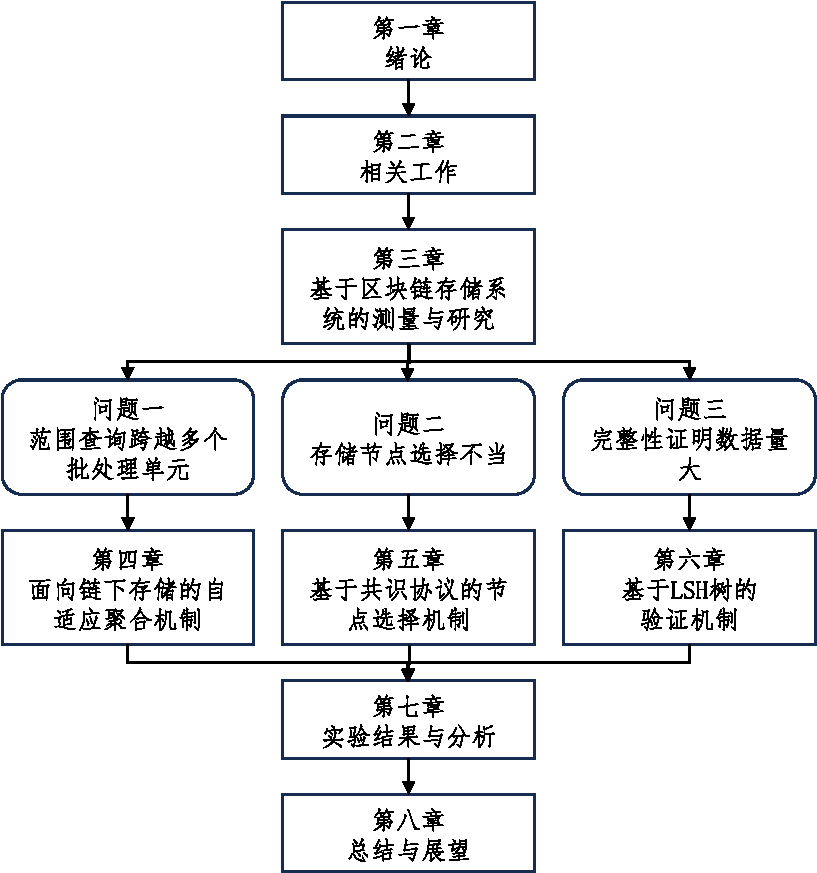
\includegraphics[width=0.8\linewidth]{timechain/roadmap.pdf}
    \caption{基于区块链的物联网时序数据高效存储技术研究内容}
    \label{fig:roadmap}
\end{figure}

围绕上述研究内容和贡献,本文将内容分为如~\autoref{fig:roadmap}所示的八个章节展开,各章节组织如下:

第一章介绍了本文的研究背景和意义,概述了本文的主要工作和贡献,以及全文的结构安排。

第二章详细回顾了分布式存储系统、区块链存储系统和聚类算法等相关技术领域,分析了现有技术在本场景下的的局限性,并探讨了区块链共识机制和验证机制在物联网数据存储中的研究进展。
进一步讨论了这些技术在实际应用中的不足之处,为本文提出的TimeChain系统提供了改进的方向和理论支持。

第三章提出了基于区块链的物联网时序数据存储系统的基础架构,并通过对系统性能的实验测量评估,揭示了现有系统的性能瓶颈。
本文进一步分析了这些瓶颈的根本原因,并提出了针对性的优化策略,提出了高效的存储技术TimeChain。
本文介绍了TimeChain的核心模块和各模块的功能,为后续章节的详细设计提供了基础。

第四章针对测量揭示的跨越多个聚合单元问题,提出了一种自适应聚合机制。
本文通过构建无向加权图和采用谱聚类算法减少查询延迟,提高了数据存储的效率。
本文也进一步讨论了该机制如何根据历史查询模式动态调整数据聚合策略,以适应不断变化的查询需求。

第五章针对测量揭示的存储节点选择错误问题,提出了一种基于共识协议的节点选择机制。
该机制综合考虑了节点信誉和传输距离,提高了节点选择的安全性和准确性,降低了数据传输延迟。
为了确保去中心化节点选择的效率,该机制将节点选择过程与共识过程相结合,以提高整个系统的抗攻击能力和可靠性。

第六章针对测量揭示的完整性验证数据较大问题,设计了一种基于LSH树的数据完整性验证机制。
本文利用物联网数据的局部相似性,使用LSH算法减少了验证过程中的数据传输量,提高了验证效率。
本文也进一步分析了LSH树在提高数据验证速度和减少网络负载方面的潜力,为物联网数据的高效验证提供了新的解决方案。

第七章实现并基于公开数据集评估了TimeChain。
本文将TimeChain与现有较为先进的解决方案进行性能对比,也通过消融实验进一步证明了TimeChain各技术点的有效性。

第八章总结了TimeChain系统的主要研究成果,并对未来的研究方向和TimeChain系统的改进进行了展望。
本文也进一步讨论了如何将TimeChain系统拓展到更广泛的应用场景,以及如何进一步提升系统性能和安全性,为后续研究提供了方向。

\chapter{相关工作}
\section{面向物联网的分布式存储系统}
近年来,随着数据规模的急剧增长和应用需求的多样化,集中式数据存储解决方案的固有漏洞逐渐显露出来,尤其是对于易受单点故障影响的局限性,引起了人们对分布式数据库的日益关注。
在传统集中式数据存储方式中,数据通常集中存储在单一节点或少数几个节点上,这种架构容易导致单点故障问题。
一旦出现故障,整个系统的稳定性和可用性将受到严重影响,甚至导致数据的不可靠或不可用。
相比之下,分布式数据库将数据分散存储在多个节点或数据中心中,这使系统本身就具备了抗单点故障的能力。
即使某个节点或数据中心发生故障,系统仍然可以继续运行并提供服务,从而保障了数据的可靠性和稳定性。
因此,随着对数据安全性、可用性和性能要求的不断提高,分布式数据库作为一种能够克服集中式存储固有弱点的解决方案,逐渐成为了当今大数据时代的主流选择。

Apache Cassandra~\cite{lakshman2010cassandra}作为一个分布式结构化键值存储系统,借鉴了Dynamo~\cite{decandia2007dynamo}的分布式系统技术和Google BigTable~\cite{chang2008bigtable}的数据模型优势,通过特殊的数据分发策略确保数据存储的高可用性和容错性。
其灵活的数据模型和分布式特性使得它适用于需要横向扩展和高性能的应用场景。

Spanner~\cite{corbett2013spanner}是谷歌开发的全球分布式数据库。
它通过TrueTime API~\cite{cervin2016truetime}提供的时间戳服务实现全球性一致性和高可用性,并结合关系型数据库的ACID属性和分布式数据库的横向扩展,适用于需要高度一致性和水平扩展的工业应用场景。

\begin{figure}[t]
    \centering
    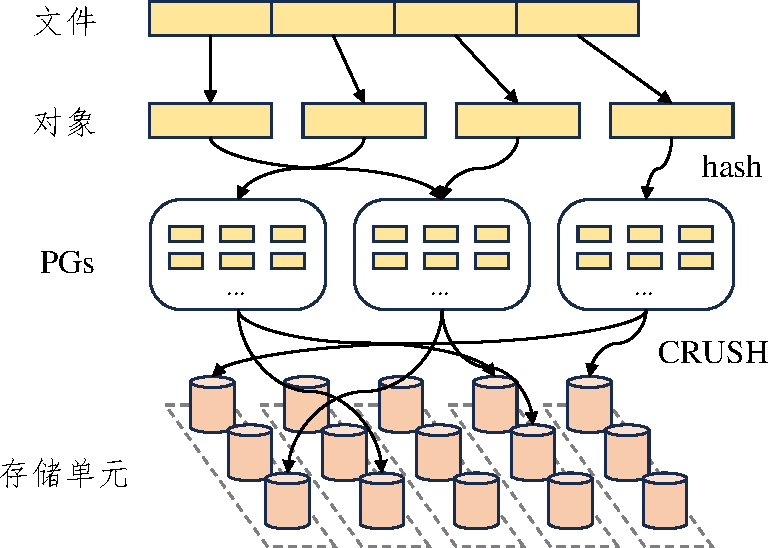
\includegraphics[width=0.6\linewidth]{timechain/ceph.pdf}
    \caption{Ceph存储流程}
    \label{fig:ceph}
\end{figure}

Ceph~\cite{weil2006ceph}作为一个开源的分布式存储系统,提供对象存储、块存储和文件系统存储功能。
为了平衡各存储节点的压力,它提出了可扩展哈希下的受控副本(Controlled Replication Under Scalable Hashing,CRUSH)算法,用于数据的分布式存储和数据冗余备份。
如~\autoref{fig:ceph}所示,对于需要被存储的文件而言,Ceph会首先将文件划分成多个独立的对象,然后Ceph将对象根据哈希分成若干放置组(Placement Group,PG)。
随后,CRUSH算法结合地理位置信息将数据对象映射到存储集群中的存储节点,实现数据的均衡分布和高效访问。
这种分布式、无中心化的数据分布方式使Ceph系统具有高度的可扩展性和容错性,即使在节点故障或网络分区的情况下,系统仍能保持数据的可靠性和可用性。

CockroachDB~\cite{taft2020cockroachdb}在Spanner的基础上,通过设计结合地理信息的复制和自动恢复机制来实现高容错性。
它将数据分布在不同的地理位置或数据中心,确保数据的冗余备份分布在不同的地理区域。
这种地理信息复制策略使得即使某个地理区域发生故障,数据仍然可以从其他地理位置的备份节点进行恢复。

然而,这些分布式存储系统仍然存在着单点故障和高存储成本的问题。
这是因为即使数据存储在不同位置,数据的管理仍然是中心化的。
在这些存储系统中,公司有可能在数据拥有者不知情的情况下轻松篡改数据,直接危及数据的完整性和安全性。
这些缺陷限制了这些系统在处理物联网数据激增和复杂协作需求方面的灵活性和效率,同时也使得数据的安全性和可靠性备受质疑。
因此,解决这些问题对于推动分布式存储系统在未来应用中获得广泛应用至关重要。

\section{基于区块链的存储系统}
根据数据的存储位置,区块链存储系统可以分为链上存储和链下存储。

\subsection{面向交易数据的链上存储}
区块链技术的出现为分布式存储系统的安全性和可靠性提供了新的解决方案。
区块链存储系统是一种基于区块链技术的分布式存储解决方案,其核心概念是将数据分布式存储在网络中的多个节点上,并使用区块链作为数据的验证和记录机制。
在区块链存储系统中,数据被分割成块,并以链式连接的方式进行存储,每个数据块包含了前一个块的哈希值,从而构成了不可篡改的数据记录链。
这种数据结构使得数据的完整性和安全性得到了极大的保障,任何尝试篡改数据的行为都会被系统所记录和拒绝。
区块链存储系统的去中心化特性意味着数据的管理不再依赖于单一实体,而是由网络中的多个节点共同维护和验证。
这种设计使得数据拥有者可以更加信任系统,因为数据的安全性和可靠性不再受限于单一实体的控制。
目前,许多链上存储的研究都集中在链上数据存储的性能上,包括查询性能和存储负担。

\begin{figure}[t]
    \centering
    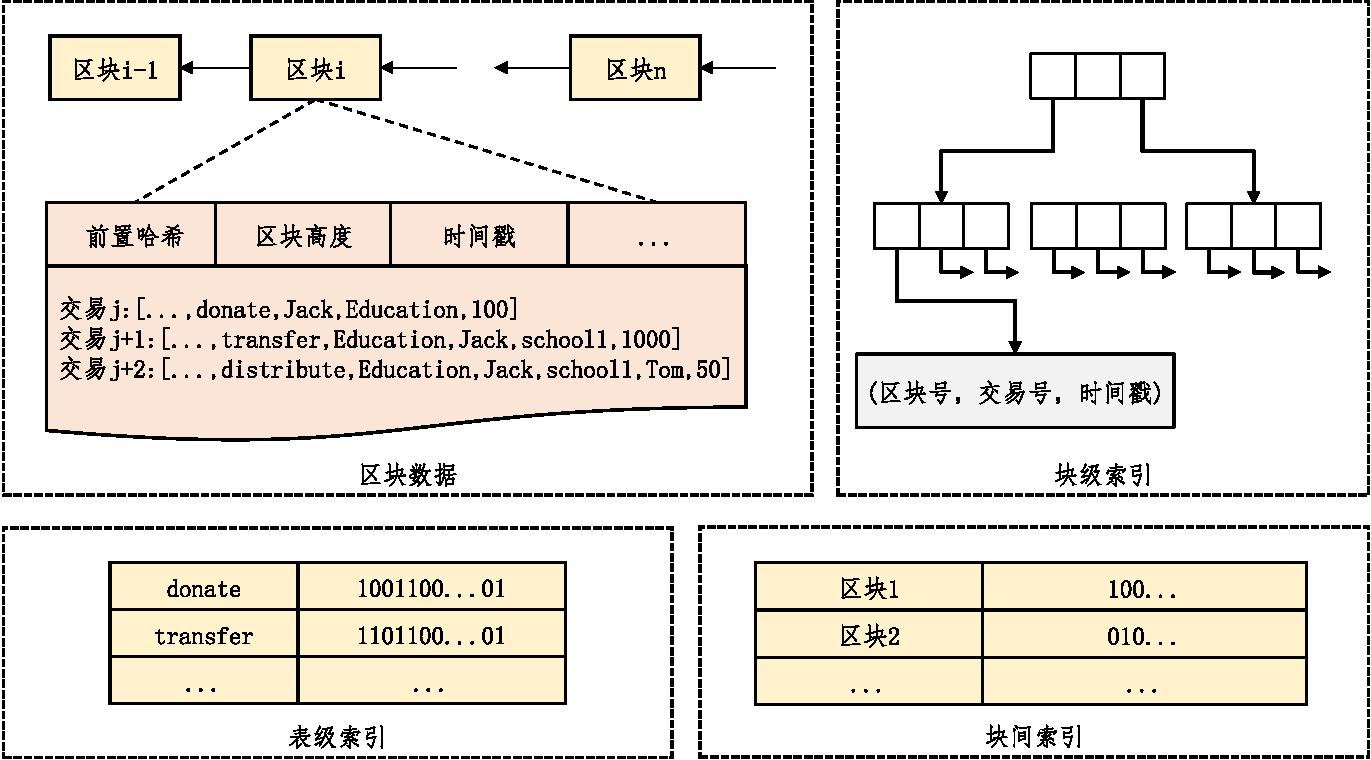
\includegraphics[width=1\linewidth]{timechain/sebdb.pdf}
    \caption{SEBDB数据结构}
    \label{fig:sebdb}
\end{figure}

部分工作关注于增强链上存储的查询支持。
由于区块链的交易数据都是以日志的形式存储在区块链上,无法提供类似关系型数据库的高效查找。
因此,一些工作提出了在区块链上建立索引的方法,以支持对区块链数据的高效查询。
% SEBDB~\cite{zhu2019sebdb}使用B+树建立了块级索引,将真实的数据组织成B+树,以支持类SQL查询。
如~\autoref{fig:sebdb}所示,SEBDB~\cite{zhu2019sebdb}使用B+树建立了块级索引,将真实的数据组织成B+树,以支持类SQL查询。
SEBDB也建立了表级索引和块间索引,便于快速定位区块位置。
MSTDB~\cite{zhou2022mstdb}则建立了基于语义的索引结构默克尔语义树(Merkle Semantic Trie,MST),以支持基于语义的多关键字查询,并对于top-k查询以及范围查询的验证方法做出优化。
MSTDB也利用索引压缩和查询预处理技术,进一步提高了存储和查询性能。

也有部分工作优化了区块上的索引和认证机制,以提高区块链状态的查询速度。
LVMT~\cite{li2023lvmt}采用了认证多点评估树(Authenticated Multipoint Evaluation Tree,AMT)在常数时间内更新完整性证明,并且采用多层设计来支持无限的键值对。
LVMT还通过存储版本号替代哈希的方式避免了昂贵的椭圆曲线乘法运算。
COLE~\cite{zhang2024cole}基于学习索引和列存储优化了区块链的存储索引结构。
COLE将数据按状态地址连续存储,通过学习索引模型减少存储索引开销;并针对区块链的存储磁盘特性引入了LSM树,以支持高效的读写性能。

部分工作关注链上存储的性能优化。
FalconDB~\cite{peng2020falcondb}和Chen等人提出的仲裁模型~\cite{chen2022blockchain}都关注区块链节点之间数据交互的效率。
为了减轻区块链账本数据存储的负担,Rapidchain~\cite{zamani2018rapidchain}、SlimChain~\cite{xu2021slimchain}和GriDB~\cite{hong2023gridb}将账本的数据分配给其他分片存储,以减轻存储压力。

在大规模数据生成迅速的物联网场景中,上述解决方案存在两方面的挑战。

\begin{itemize}
    \item[$\bullet$] 首先,这些解决方案会给区块链带来额外的空间存储负担。
    由于物联网设备在短时间内生成的数据量庞大,将这些数据全部存储在区块链上可能会导致链的存储需求急剧增加,进而增加系统的复杂性和成本。
    \item[$\bullet$] 其次,这些方案可能导致数据隐私泄露的风险增加,因为在区块链上存储的数据通常是不可篡改和公开可见的,这会导致物联网的数据泄露。
\end{itemize}

综上所述,在数据密度低、生成速度快的物联网场景下直接使用传统的链上存储方案,会产生较大的开销和风险。
物联网场景需要更加注重数据存储效率和隐私保护,因此需要针对这些特殊需求设计更为灵活和高效的数据管理方案。

\subsection{面向文件数据的链下存储}
\begin{figure}[t]
    \centering
    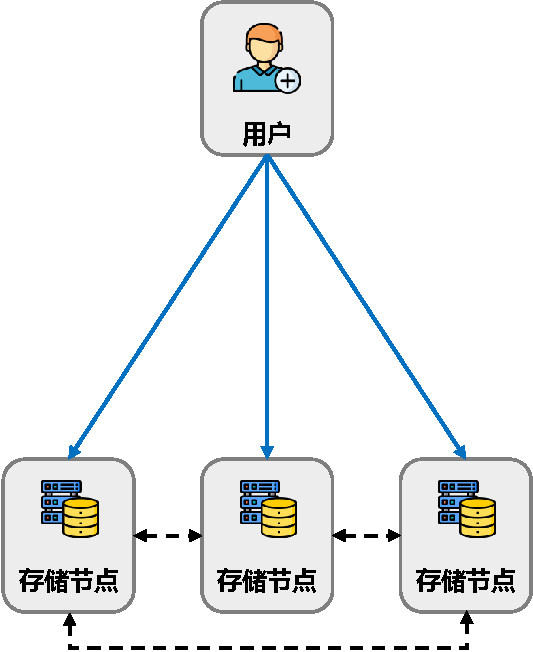
\includegraphics[width=0.7\textwidth]{timechain/filedes.pdf}
    \caption{去中心化存储系统}
    \label{fig:filedes}
\end{figure}

基于区块链的文件系统因其较少的开销而备受广泛研究和关注。
这些系统将文件本身存储在链下,规避了原始数据直接存储在链上带来的巨大开销,并通过在区块链上记录文件的哈希值和验证信息来确保文件的完整性和安全性。
由于区块链的不可篡改性,用户可以方便地验证文件的来源和完整性,防止数据篡改和丢失。
相较于传统的中心化存储系统,基于区块链的文件系统通常不需要中心化的服务器和维护成本,从而降低了整体的运营成本。

FileCoin~\cite{bauer2022filecoin}是建立在星际文件系统(InterPlanetary File System,IPFS)的去中心化文件存储系统。
IPFS是一种点对点的分布式文件系统,它通过内容寻址来存储和共享文件,使得文件在没有单点故障的分布式网络上可用。
通过激励机制鼓励用户提供存储服务,FileCoin利用区块链技术确保了文件的完整性和可靠性,同时为用户提供了一种去中心化的存储解决方案。
如图~\ref{fig:filedes}所示,在FileCoin中,节点可以通过提供存储空间来获取FileCoin代币奖励,从而构建一个分布式的文件存储网络。
对于这个完全去中心化的系统而言,所有存储节点之间都是平等的,每个节点将参与到用户的请求处理过程中。
这种模式不仅激励了更多的存储资源加入网络,还提高了数据的持久性和可访问性,因为文件被分散存储在全球各地的节点上,减少了中心化存储的风险。
为了确保文件的完整性,FileCoin为每个文件建立默克尔树,通过分散存储文件块来提高可靠性和安全性,从而降低了数据丢失的风险。
用户可以通过这些系统安全地存储和共享文件,同时保持数据的隐私和安全性。

\begin{figure}[t]
    \centering
    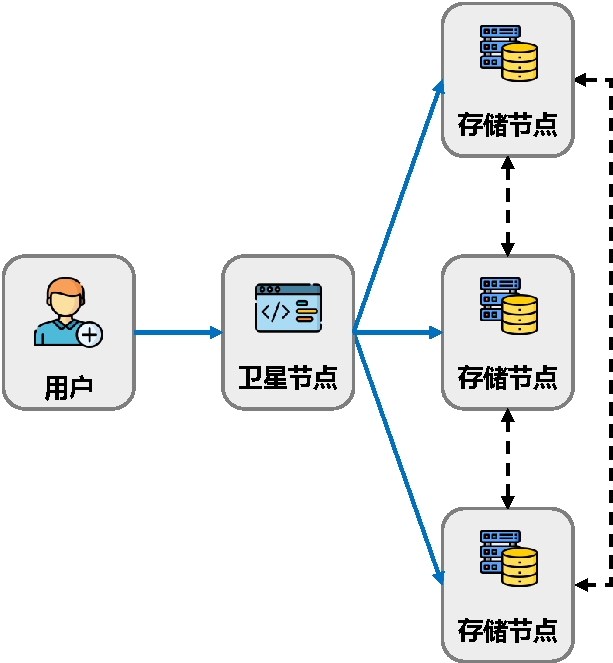
\includegraphics[width=0.7\textwidth]{timechain/storj.pdf}
    \caption{半去中心化存储系统}
    \label{fig:storj}
\end{figure}

Storj~\cite{storj2018storj}和Sia~\cite{vorick2014sia}是两个典型的半去中心化的文件存储系统。
如图~\ref{fig:storj}所示,在半去中心化网络中,除了存储节点,也存在一组卫星节点。
这些卫星节点通过运行特定的智能合约来处理用户的请求,例如选择存储节点、进行文件切分、索引文件等。
他们也为每个文件建立默克尔树以确保文件的完整性。

FileDES~\cite{xu2024filedes}专注于数据的加密存储,借助零知识证明等技术来保护数据的安全性。
通过加密存储数据,FileDES可以确保用户的数据在存储和传输过程中不会被泄露或篡改。
这种方法为用户提供了更高级别的数据安全保障,尤其适用于对数据隐私和安全性要求较高的场景。

然而,尽管这些方法在确保文件完整性和安全性方面表现出色,它们并不适用于高效存储物联网数据的存储。
这是因为物联网数据通常具有较低的价值密度,而将单个数据以文件形式存储在区块链文件系统中,将导致极高的成本。
物联网数据的特点决定了需要更为轻量级和高效的数据存储方案,以更好地应对数据生成量大、频繁性高的特点,同时降低存储和处理成本。
因此,对于物联网大规模数据存储的需求,寻找轻量、高效、可信的数据解决方案是一个挑战。

\section{本章小结}
在本章中,本文广泛探讨了面向物联网的分布式存储系统和基于区块链的存储系统的相关研究工作。
本文分析了集中式数据存储解决方案的局限性,特别是它们在面对单点故障时的脆弱性,以及分布式数据库如何通过在多个节点间分散存储数据来提高数据的可靠性和稳定性。
本文详细讨论了Apache Cassandra、Spanner、Ceph和CockroachDB等分布式存储系统,它们通过不同的技术手段实现了数据的高可用性和容错性。
然而,这些系统仍然存在单点故障的风险,并且由于数据管理的中心化,数据的完整性和安全性仍然受到威胁。

进一步地,本文探讨了基于区块链的存储系统,它们通过将数据分布式存储在多个节点上,并利用区块链作为数据验证和记录的机制,提供了一种新的数据存储解决方案。
本文分析了链上存储和链下存储两种方法,以及它们在提高数据存储性能和确保数据完整性方面的研究进展。
尽管这些基于区块链的存储系统在确保数据完整性和安全性方面具有优势,但它们在处理大规模、低价值密度的物联网数据时面临效率和成本的挑战。

综上所述,现有的分布式存储系统和基于区块链的存储系统虽然在某些方面取得了进展,但它们在满足物联网数据存储需求方面仍存在不足。
这些挑战包括处理大规模数据的效率、数据存储的成本以及数据隐私保护的需求。
因此,开发一种轻量级、高效且可信的数据存储解决方案对于物联网领域来说是一个重要的研究方向。
TimeChain系统正是在这样的背景下应运而生,旨在结合区块链技术的优势,解决物联网时序数据存储中的关键问题。

\chapter{基于区块链存储系统的测量与研究}
\label{sec:baseline}
本章将深入探讨基于区块链的物联网时序数据存储系统的基础架构,并对该系统进行了全面的测量研究。
基于测量研究,本文发现聚合存储能够显著降低存储延迟,但在物联网场景中较为常见的范围查询中,同时也引入了查询延迟的问题。
本章进一步分析了导致查询性能不佳的根本原因,包括查询跨越多个聚合单元、存储节点选择不当以及庞大的数据完整性证明。
为了解决这些问题,本文提出了TimeChain架构,这是一种新颖的、基于区块链的物联网时间序列数据存储系统。
本章介绍了TimeChain系统的核心模块,包括数据批处理模块、存储节点选择模块和数据验证模块。
这些模块共同作用,旨在减少查询延迟、提高数据存储的效率和安全性。

\section{基于区块链存储系统的架构}

\begin{figure}[t]
    \centering
    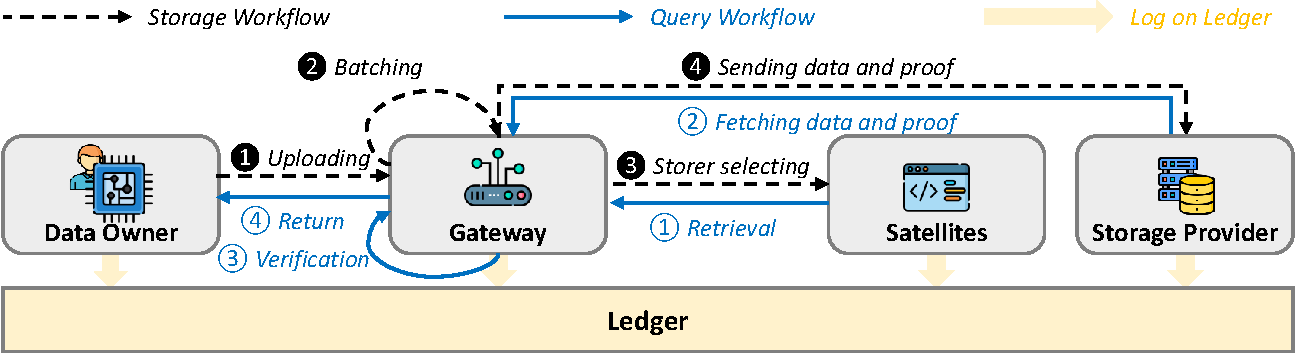
\includegraphics[width=0.8\linewidth]{timechain/measurement_workflow.pdf}
    \caption{基于区块链的存储系统的工作流}
    \label{fig:workflow}
\end{figure}

为了提高基于区块链的分布式数据库的性能,本文提出了一种基本的链下存储系统,并对其进行了测量研究。
如~\autoref{fig:workflow}所示,一个基于区块链的基本分布式存储系统有四个主要角色,即\textbf{数据拥有者}、\textbf{网关}、\textbf{卫星}和\textbf{存储提供商}。

\begin{itemize}
    \item[$\bullet$] \textbf{数据拥有者}:数据拥有者是数据的生成者和消费者,他们发起上传和查询数据的请求。
    \item[$\bullet$] \textbf{网关}:网关是数据拥有者与存储提供商之间的中间层,负责数据的上传和下载。
    \item[$\bullet$] \textbf{卫星}:与Storj~\cite{storj2018storj}和FileCoin~\cite{bauer2022filecoin}类似,卫星是一个智能合约,负责协调数据拥有者和存储提供商之间的交互。
    它们提供文件审计(检查)或可检索性(Proofs of Retrievability,POR)相关功能和对存储支付等操作的处理。
    \item[$\bullet$] \textbf{存储提供商}:存储提供商是存储数据的节点,通过提供存储服务获得奖励。
    为了使存储提供商能够通过灵活的查询快速向数据拥有者提供完整性证明,数据完整性证明也需要存储在存储提供商中,便于通过默克尔树的路径直接快速组装成完整性证明。
    存储提供商的服务信息,如剩余存储空间,将与交互记录一起记录在分布式账本中,以确保安全。
\end{itemize}

一般来说,数据存储和查询过程可以概括如下:

\textbf{数据存储:}
\ding{182}\textit{上传}:
数据拥有者通过网关接口上传数据。
\ding{183}\textit{聚合}:
网关接收到数据后,会对时间序列数据进行批处理。
这一步骤涉及到将多个数据点聚合在一起,并为每批数据生成数据完整性证明,这对于确保数据在存储和后续查询过程中的完整性至关重要。
\ding{184}\textit{选择存储节点}:
在聚合数据后,卫星节点介入,帮助网关识别和选择最佳的存储节点。
这一步骤基于一系列选择标准,如节点的信誉、存储空间和地理位置等,以确保数据被存储在最可靠和最经济的节点上。
\ding{185}\textit{发送数据和完整性证明}:
一旦确定了最佳存储节点,原始传感器数据及其完整性证明将被发送到这些节点。
同时,数据批的元数据被记录在分布式账本中,利用区块链的不可篡改性确保数据的透明性和可追溯性。

\textbf{数据查询:}
\ding{172}\textit{检索}:
当数据拥有者需要访问他们的数据时,他们通过网关发起数据下载请求。
网关随后与卫星节点交互,以检索存储提供商的位置信息。
\ding{173}\textit{获取数据和完整性证明}:
网关根据从卫星节点获得的位置信息,从存储提供商处获取所需的数据及其完整性证明。
这一步骤确保了数据在传输过程中的安全性和完整性。
\ding{174}\textit{验证}:
在获取数据后,网关将通过检查数据完整性证明来验证下载数据的完整性,确保数据未被篡改且准确无误。
\ding{175}\textit{返回}:
最后,经过验证的数据将通过网关安全地返回给数据拥有者,完成整个数据查询流程。

\section{基于区块链存储系统的测量}
在本节中,本文进行了一项初步测量,以评估基于区块链的基本存储系统的性能。
本文基于Hyperledger Fabric实现了上述存储系统。
该测试网络由5个节点组成,其中1个节点是网关,4个节点是卫星。
为了更准确地模拟真实世界中的存储网络环境,本文基于真实世界的数据存储网络模拟了一个包括320个存储节点的网络,其中包括189个真实存储提供商~\cite{corneo2021surrounded}和131个模拟提供商(代表提供闲置存储的个人提供商)。
为了确保实验结果的准确性,网关与这些模拟提供商之间的传输延迟是通过一个基于现有研究的线性回归模型~\cite{ziviani2005improving}进行预测的。
\begin{figure*}[t]
    \centering
    \begin{minipage}{1\linewidth}
	    \centering
        \subfloat[存储时延]{
            \centering
            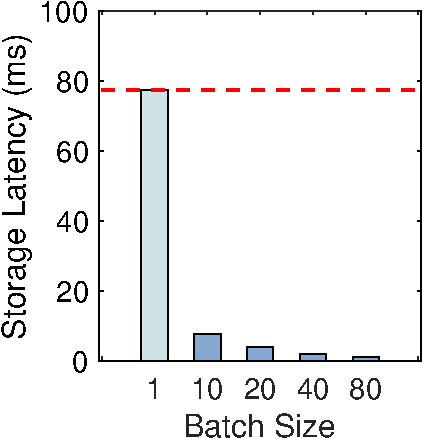
\includegraphics[width=0.45\textwidth]{timechain/measurement_storage.pdf}
            \label{fig:measurement_storage}
        }
        \hfill
        \subfloat[查询时延]{
            \centering
            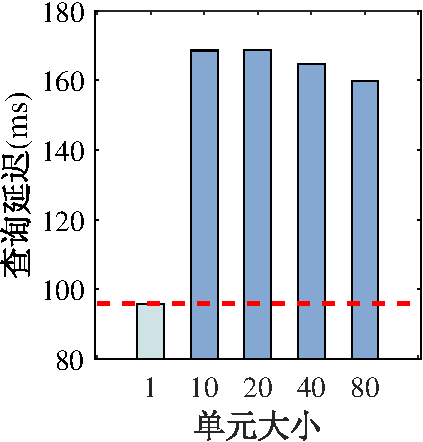
\includegraphics[width=0.45\textwidth]{timechain/measurement_query.pdf}
            \label{fig:measurement_query}
        }
        \caption{区块链存储系统的性能} 
    \end{minipage}
\end{figure*}

\textbf{存储性能。}
在本文设置的系统中,数据拥有者每秒生成20个56字节的数据包,并在20秒内存储它们。
存储性能结果如图~\autoref{fig:measurement_storage}所示。
与单独存储每个数据相比,批存储将延迟减少到约37.4分之一,且随着聚合单元增大,存储延迟逐渐降低。
这主要是因为较大的聚合单元规模减少了链上操作和数据传输的次数,从而降低了存储延迟。

\textbf{查询性能。}
然后,本文测试范围查询的性能,如图~\autoref{fig:measurement_query}所示。
不幸的是,结果显示,相对于存储单个数据而言,批处理存储解决方案的查询性能相对较差。
批量存储在不同聚合单元大小下的平均延迟为165.4ms,无法满足许多物联网场景的需求。
例如,自动驾驶应用程序的延迟小于50ms~\cite{caesar2020nuscenes},地震监测的延迟小于100ms~\cite{bhatia2023artificial}。

\section{性能瓶颈的根本原因}
为了找出该方案查询性能不佳的原因,本文进行了深入研究,并将原因总结为以下三点:

\begin{figure*}[t]
    \centering
    \begin{minipage}{1\linewidth}
	    \centering
        \subfloat[查询跨越多个batch]{
            \centering
            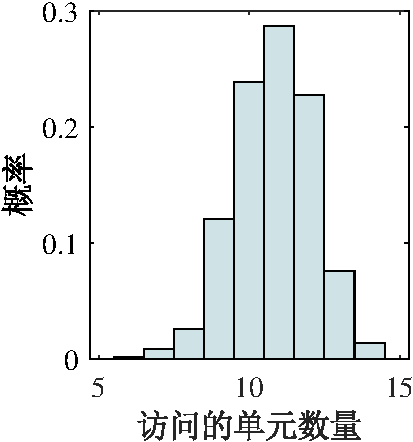
\includegraphics[width=0.3\textwidth]{timechain/batch_cdf.pdf}
            \label{fig:batch_cdf}
        }
        \hfill
        \subfloat[不正确的存储节点选择]{
            \centering
            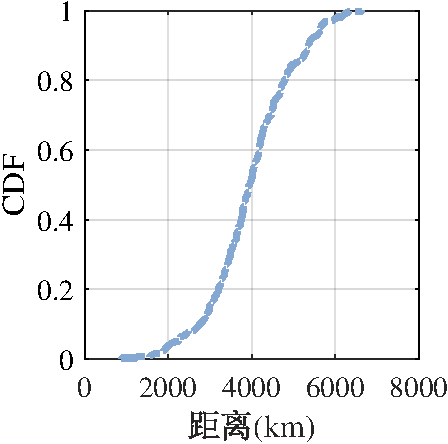
\includegraphics[width=0.3\textwidth]{timechain/dis_cdf.pdf}
            \label{fig:dis_cdf}
        }
        \hfill
        \subfloat[传输数据较大]{
            \centering
            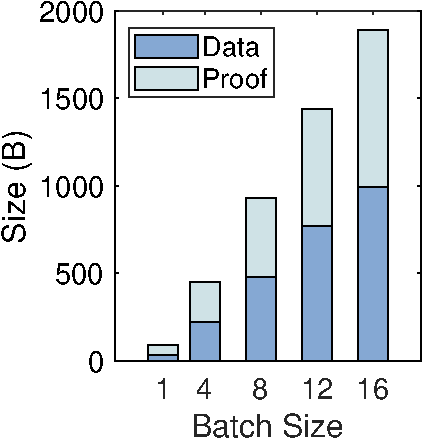
\includegraphics[width=0.3\textwidth]{timechain/proof_size_cdf.pdf}
            \label{fig:proof_size_cdf}
        }
        \caption{性能低下的根本原因} 
    \end{minipage}
\end{figure*}

\begin{enumerate}
    \item \textbf{范围查询跨越多个批处理单元。}
    时间序列数据的查询通常包含多个数据点,如范围查询、聚合查询、过滤查询等。
    如果批处理不当,单个查询可能会跨越多个批处理单元。
    本文使用现有的数据集YCSB~\cite{barata2014ycsb}评估每个查询所跨越的批处理单元数量。
    如图~\autoref{fig:batch_cdf}所示,超过84.25\%的查询跨越了10个批处理单元。
    当这些批处理单元被存储在不同的节点上时,将引入额外的查询和传输延迟。

    \item \textbf{存储节点选择不当。}
    在这个测量中,本文发现传输延迟占总查询延迟的很大一部分。
    如图~\autoref{fig:dis_cdf}所示,世界各地存储节点的距离存在很大差异,导致节点之间的传输延迟存在很大差异。
    如果选择非常远的存储节点,传输延迟将会显著增加。
    此外,在整个存储网络中存在恶意节点的情况下,尽管最终选择的节点可能传输延迟较小,然而,由于恶意节点的存在,数据的完整性可能会受到威胁,从而无法提供完整的数据存储服务。

    \item \textbf{完整性证明数据量大。}
    为了使存储提供商能够通过灵活的查询快速向数据拥有者提供完整性证明,数据完整性证明也需要与存储提供商一起存储。
    因此,当存储提供商需要向数据拥有者证明数据的完整性时,完整性证明也会被发送回数据拥有者。
    图~\autoref{fig:proof_size_cdf}显示了总传输数据量的各组成部分。
    从图中可以看出,数据完整性证明大小占接收数据的48.8\%,几乎是接收数据的一半。
    当网络繁忙时,大量的完整性证明数据传输会增加网络传输延迟。
\end{enumerate}

\section{高效的链下存储架构}
\label{sec:design}

\begin{figure}[t]
    \centering
    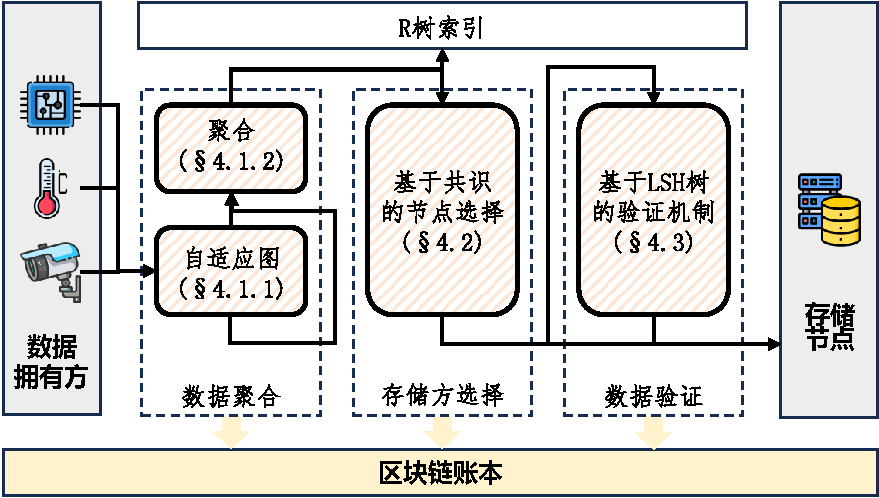
\includegraphics[width=0.9\linewidth]{timechain/arch.pdf}
    \caption{TimeChain架构}
    \label{fig:architecture}
\end{figure}

为了提高区块链存储系统的查询性能,本文设计了一种基于区块链的新型物联网时间序列数据存储系统,TimeChain。
\autoref{fig:architecture}显示了TimeChain的架构。
TimeChain中的模块包括数据聚合、存储方选择、数据验证、R树索引和区块链账本。
TimeChain建立在区块链平台上,所有操作都记录在分布式账本上,以方便数据的审计和追踪。
TimeChain的索引结构是R树,可以加速物联网场景中常用的时空聚合搜索。
原始数据经过数据聚合模块,确定哪些数据被放在一个聚合单元中;经过存储方选择模块,确定聚合单元的存储位置。
这些信息将被放在R树中,以便快速查询。
接下来,本文介绍TimeChain的关键模块。

\textbf{数据聚合模块:}
本文的测量研究表明,不正确的聚合方法会增加查询的跨单元数量,从而增加网络传输延迟。
本文构建了一个自适应的无向加权图(Undirected Weighted Graph,UWG),以基于数据拥有者的历史查询准确捕获用户查询信息(§-\ref{sec:UWG})。
基于本文构建的UWG,本文将数据打包成批处理单元的问题转换为聚类问题~\cite{xu2005survey},该问题根据用户的查询请求将所有原始数据划分为多个聚类。
解决聚类问题的传统算法有很多,如K-means~\cite{kanungo2002efficient}、GMM~\cite{he2010laplacian}等。
然而,这种传统的聚类算法不适合分割物联网设备生成的数据。
这是因为在TimeChain中,用户的查询没有遵循特定的特征,这可能会导致数据图的聚类形成复杂的形状,而不是常见的圆形。
此外,传统的聚类算法需要将所有数据划分为固定数量的集合,但并非所有集合都等于批大小,这将给索引查询带来额外的开销。
因此,本文使用谱聚类算法来打包数据(§-\ref{sec:ratiocut}),这非常适合处理不规则和非固定数量的聚类。

\textbf{存储方选择模块:}
存储节点的\textit{选择}至关重要。
正如本文之前在图~\autoref{fig:dis_cdf}中发现的那样,存储节点和网关之间的距离会影响数据访问延迟。
此外,对于链下存储系统,存储空间不足的节点或恶意节点可能会导致数据丢失、篡改或服务中断,进而影响整个系统的安全性和稳定性。
因此,本文根据距离和历史服务记录等信息对存储节点进行综合评估。
存储节点\textit{选择过程的安全性}也非常重要。
Storj~\cite{storj2018storj}、CoopEdge~\cite{yuan2021coopedge}和PipeEdge~\cite{yuan2023pipeedge}通过一组固定的节点选择服务节点,并通过区块链确认决策。
换句话说,他们集中决策,但仍然面临单点失败的威胁。
然而,使用类似于PBFT的投票机制,节点选择过程通常需要多轮任务计算和消息广播。
如果共识过程和节点选择过程完全解耦,系统安全将受到威胁。
为了解决这个问题,本文将节点选择过程与共识相结合,提出了一种基于共识的节点选择机制(§-\ref{sec:consensus})。

\textbf{数据验证模块:}
从之前的测量结果中本文可以发现,传输的数据中接近一半是数据完整性证明。
数据完整性证明被组织为默克尔树的形式,它是由一系列哈希构建的。
在默克尔树中,非叶子节点的哈希数几乎等于原始数据点的数量。
由于物联网数据单元的大小大约等于哈希值,这意味着需要发送以验证数据的数据量几乎是原始数据的两倍。
在这样的数据传输过程中,减小数据证明的大小是一个挑战。
通过分析物联网数据,本文观察到物联网数据变化缓慢,在短时间内很少出现突然变化。
对于这些相似的数据,LSH算法可以从相似的原始数据中生成相似的哈希结果。
LSH算法确保类似的物联网数据即使在哈希后也保持相似。
因此,本文提出了一种新的基于LSH树的验证机制(§-\ref{sec:lsh}),该机制采用LSH而不是传统默克尔树中使用的通用哈希。
通过差分传输LSH哈希值,可以显著减小传输数据的大小。

\section{本章小结}
在本章中,受链下存储启发,本文先提出了一种基于区块链的物联网时序数据基本存储系统。
对于这个基本系统,本文进行了一些性能测试,发现该系统确实可以降低存储延迟,但查询延迟较高。
本章进一步分析了查询性能不佳的根本原因,并针对性能瓶颈提出了高效链下存储系统TimeChain的架构。
对于跨越多个聚合单元问题,本文在聚合阶段提出了一种自适应聚合机制。
对于存储节点选择错误问题,本文在节点选择阶段提出了一种基于共识协议的节点选择机制。
对于完整性验证数据较大问题,本文在验证阶段设计了一种基于LSH树的数据完整性验证机制。
本文将在后续段落中进一步介绍这三个机制的设计。

\chapter{面向链下存储的自适应聚合机制}
\label{sec:packaging}
本文的测量结果揭示了一个关键问题:不当的数据聚合策略会导致查询过程中需要跨越更多存储单元,进而增加了网络传输的延迟。
在本章中,本文提出了一种自适应UWG的方法,它能够根据数据所有者的历史查询模式精确捕捉用户的查询行为。
利用这个自适应UWG,本文将数据分批的问题转化为一个聚类问题,即根据用户的查询需求将海量原始数据划分成多个有意义的聚类。

尽管存在多种传统的聚类算法,例如K-means和GMM,它们不适合处理物联网设备产生的数据时。
原因在于TimeChain系统中用户查询的模式多样化,不遵循统一特征,这可能导致聚类结果呈现出不规则的形状,而非典型的圆形。
此外,这些传统算法通常要求将数据均匀分配到固定数量的聚类中,这与本文的需求不符。
因为不是所有的聚类都恰好匹配一个批次的大小,这无疑会增加索引查询的负担。

\section{基于历史查询的自适应图构建过程}
\label{sec:UWG}

\begin{table}
    \centering
    \caption{TimeChain关于聚合的符号和定义}
    \begin{tabular}{|c|c|}
        \hline
        \textbf{符号} & \textbf{描述} \\
        \hline
        $d_i$   & 第$i$个设备 \\
        \hline
        $D$     & 所有设备集合,$D = \{d_0, ..., d_n\}$\\
        \hline
        $s_i$   & 物联网传感器产生的第$i$条数据 \\
        \hline
        $S$     & 所有数据集合,$S = \{s_0, ..., s_m \}$\\
        \hline
        $Q^i$   & 第$i$条用户查询集合,$Q^i = \{ q_0, ..., q_r \}$\\
        \hline
        $q_k$   & $k$中的第$Q^i$条查询 \\
        \hline
        $l_{ab}$& 查询权重包含设备$a$和设备$b$ \\
        \hline
        $L$     & 一起查询的数据权重,$L = \{l_{ab} | \exists_{a,b} \in D \}$\\
        \hline
        $x^k_{ab}$ & 设备$a$和设备$b$是否同时被查询 \\
        \hline
        $X^k$   & 设备访问信息,$X^k = \{x^k_{ab} | \exists_{a,b} \in D \}$\\
        \hline
        $P$     & 数据打包结果,$P = \{ \{ s_i, ... \}, ... \}$\\
        \hline
    \end{tabular}
    \label{tab:notations}
\end{table}

由于物联网的原始数据是孤立的点,本文在数据点之间创建加权边,表示被联合查询的概率。
数据点$a$和$b$之间的边的权重$l_{ab}$表示为:

\begin{equation} 
    \label{eq:weight}
    \begin{split}
        l_{ab} =
        \begin{cases}
            \sqrt{ (id_a - id_b)^2 + (t_a - t_b)^2 } &, k = 0 \\  
            \theta \cdot l_{ab} + (1 - \theta) \cdot x_{ab}^k &, k \geq 1  
        \end{cases}
    \end{split}
\end{equation}

其中$l_{ab}$被初始化为两个数据点设备ID和数据到达时间之间的欧氏距离。
当用户的请求到达时,UWG会根据请求中涉及的数据查询范围进行动态调整。
为了避免查询图的过度存储开销,本文在更新图时忽略了数据的时间维度,只考虑数据的设备ID维度。
本文使用变量$x_{ab}^k$来指示第$k$个查询的内容。
当第k个查询包含设备$d_a$和设备$d_b$时,$x_{ab}^k=1$,否则$x_{1b}^k=0$。
然后,距离$l_{ab}$将根据$x_{ab}^k$进行更新。

由于用户请求可能非常随机,因此图的更新和变化可能会非常频繁。
因此,本文设置了一个影响因子$\theta$来确定用户请求对图更新的影响。
当$\theta$接近1时,权重受查询的影响更大。
当$\theta$接近0时,这意味着图尽可能保持初始状态。
同时,TimeChain使用滑动窗口动态更新UWG,尽可能避免单个查询的对系统的鲁棒性影响。
虽然查询模式的突然变化最初会降低打包准确率,但系统会在多次查询后快速适应。
通过自适应权重聚类算法,本文可以根据节点之间的距离和查询的相关性动态调整节点之间的权重,以更好地反映它们的相似性。
这有助于在打包过程中更准确地确定哪些节点的数据应放置在同一批中,以提高查询的效率和准确性。

\section{\tyxcmt{基于谱聚类算法的封装机制}}
\label{sec:ratiocut}

\subsection{聚类算法选择}
通过建立自适应的UWG,本文将数据分批的问题转化为聚类问题。
本文综合考虑了目前的几类聚类算法:基于划分的算法、基于模型的方法以及基于图论的方法。

\textbf{基于划分的算法。}
基于划分的算法通过迭代优化过程,将数据集划分为预定义数量的簇。
这类算法中最著名的是K-means~\cite{kanungo2002efficient}。
K-means算法首先随机选择$k$个点作为初始质心,然后将每个数据点分配给最近的质心所在的簇,并重新计算每个簇的质心。
这个过程不断重复,直到质心不再显著变化或达到最大迭代次数。
尽管这种方法简单直观且计算效率较高,但它对簇的数量$k$非常敏感,初始质心的选择也会影响最终结果。
此外,K-means假设簇是球形分布的,难以处理非球形簇或复杂形状的数据。
因此,对于TimeChain输入的时间序列数据,这些算法可能无法有效捕捉数据的真实分布,导致聚类效果不佳。

\textbf{基于模型的方法。}
基于模型的方法通过假设数据是由特定的概率分布生成的,并使用统计模型进行参数估计来实现聚类。
最典型的方法,例如高斯混合模型~\cite{kanungo2002efficient}(Gaussian Mixture Models, GMM),通过迭代地更新每个数据点属于各个高斯分布的概率,以及各个高斯分布的均值、协方差矩阵等参数,逐步优化模型,直到收敛。
虽然GMM能够提供概率解释并适用于特定类型的分布,但其计算复杂度较高,特别是在处理大规模数据集时,需要大量的计算资源和时间。
对于物联网设备来说,由于资源受限(如内存、CPU性能),这种复杂的计算对于弱性能设备而言难以承受,从而影响系统的实时性和响应速度。
另一种基于模型的方法是隐马尔可夫模型~\cite{he2010laplacian}(Hidden Markov Model, HMM),假设数据是由隐藏状态序列生成的,通过训练HMM模型,可以发现隐藏状态的转换模式,从而实现聚类。
然而,HMM的训练过程同样涉及复杂的概率计算,特别是当状态空间较大时,计算复杂度会显著增加。
因此,尽管这些方法在某些场景下非常有效,但在TimeChain的应用中并不理想,因为它们不适合资源受限的物联网环境。

\textbf{基于图论的方法。}
基于图论的方法,特别是谱聚类~\cite{von2007tutorial}(Spectral Clustering),利用图的拉普拉斯矩阵的特征向量来进行聚类,非常适合处理复杂的簇结构。
谱聚类的基本思想是将数据点表示为图中的顶点,顶点之间的边权重表示数据点之间的相似性或距离。
具体来说,首先根据数据点之间的相似性或距离度量构建一个加权图,其中每个节点代表一个数据点,边的权重表示节点之间的相似性。
接下来,从相似性图中计算出图的拉普拉斯矩阵。
拉普拉斯矩阵是一种特殊的矩阵,反映了图的拓扑结构和节点之间的关系。
随后,对拉普拉斯矩阵进行特征分解,提取前几个最小的非零特征值对应的特征向量。
这些特征向量捕获了图的主要结构信息。
最后,将提取的特征向量作为新的低维表示,应用传统的聚类算法(如K-means)进行聚类。
谱聚类不仅能够发现任意形状的簇,而且相对GMM和HMM而言,其计算复杂度是可以接受的,特别适合处理大规模数据集。
此外,谱聚类在处理噪声数据和不规则形状的簇方面表现优异。
因此,TimeChain选择了谱聚类算法进行聚类分析,以高效地处理物联网时序数据,并确保在资源受限的环境中也能保持良好的性能。

\subsection{数据封装过程}
\begin{algorithm}[t]
	\caption{聚合算法}
	\label{algo:package}
    \begin{algorithmic}[1]
        \REQUIRE 输入设备集$D$,数据集$S$,用户的历史查询集$Q^i$
        \ENSURE 最优聚合结果$P$
        \STATE $S' \gets \{s^a | a \in D \And s^a \subset S\}$ //根据设备ID梳理原始数据
        \STATE $L \gets \Big\{ \sqrt{ (id_a - id_b)^2 + (t_a - t_b)^2 } \Big| \exists_{a,b \in D} \Big\}$ //根据\autoref{eq:weight}初始化权重集$L$
        \STATE $X^k \gets \{0 | \exists_{a,b \in D} \}$ //将用户查询请求信息$Q^{i-1}$打包成集合$X^k$
        \FOR{$q^k \in Q^{i}$}
            \IF{$a,b \in q^k$}
                \STATE \textnormal{使用$x^k_{ab} \gets 1 $更新$X^k$} //将用户查询请求信息$Q^{i-1}$打包成集合$X^k$
            \ENDIF
        \ENDFOR
        \STATE $L \gets \Big\{ \theta \cdot l_{ab} + (1 - \theta) \cdot x_{ab}^k \Big| \exists_{a,b \in D} \exists_{l_{ab} \in L} \Big\}$ //更新UWG的权重集$L$
        \STATE $D' \gets \textit{cluster}(D, L)$ //使用谱聚类算法获得聚合结果$D'$
        \STATE $P \gets \{\}$ //初始化聚合结果$P$
        \FOR{$d^j \in D'$}
            \STATE \textnormal{增加$\{ s^a | \exists_{a \in d^j} \}$到$P$中} //将设备数据合并到$P$中
        \ENDFOR
        \STATE \textbf{return} $P$
    \end{algorithmic}
\end{algorithm}

\tyxcmt{展开介绍算法}
\ref{algo:package}显示TimeChain的整个打包过程。
该算法的输入包括输入设备集$D$、数据集$S$和用户的历史查询集$Q^i$。
本文首先根据设备ID和时间单位将原始数据$S$组织到一个集合$S'$中,该集合以时间单位表示设备的数据(第1行)。
本文根据\autoref{eq:weight}初始化权重集$L$(第2行)。
对于上一个滑动窗口中的历史查询记录集合$Q^{i-1}$,本文将用户查询请求信息打包成集合$X^k$(第4-8行)。
然后,本文根据收集到的查询信息$X^k$更新权重集$L$(第9行)。
对于UWG$(D,L)$,本文使用谱聚类算法来获得聚合结果$D'$(第10行)。
根据聚合结果$D'$,本文将设备数据合并到$P$中,这是本文得到的聚合结果(第12-14行)。

\section{本章小结}
在本章中,本文深入研究了面向链下存储的自适应聚合机制,旨在解决物联网时序数据存储中的查询延迟问题。
本文发现,不当的数据聚合策略会导致查询过程中需要跨越更多存储单元,从而增加了网络传输的延迟。
为此,本文提出了一种基于历史查询的自适应无向加权图(UWG)方法,该方法能够精确捕捉用户的查询行为,并根据这些行为将数据分批处理,以优化查询效率。
本文还提出了一种基于谱聚类算法的封装机制,以更好地处理不规则形状的数据聚类问题。
通过这种方法,本文可以更准确地确定哪些节点的数据应放置在同一批中,以提高查询的效率和准确性。

\chapter{基于共识协议的节点选择机制}
\label{sec:consensus}
确定最佳的存储节点选择是构建高效区块链存储系统的关键一环。
根据本文测量中的分析,如图~\autoref{fig:dis_cdf}所示,存储节点与网关之间的距离对数据访问延迟有着直接的影响。
此外,在链下存储环境中,节点存储空间不足或恶意行为可能会导致数据的丢失、被篡改或服务中断,这些都会对系统的安全性和稳定性造成严重影响。
因此,如何选择最佳的存储节点是一个挑战。

\section{中心化节点选择}
在区块链和分布式存储系统中,存储节点的选择是确保数据安全性和可靠性的关键步骤。
目前,许多系统如Storj~\cite{storj2018storj}、CoopEdge~\cite{yuan2021coopedge}和PipeEdge~\cite{yuan2023pipeedge}根据节点的信誉选择存储节点,通过区块链来确认节点选择的决策。
鉴于PBFT共识算法在分布式系统中的普遍应用,本文将阐述一个基于PBFT算法的去中心化存储系统中节点选择的具体步骤和流程。
对于一个具有$3f+1$个节点的网络中,PBFT共识协议要求至多存在$f$个恶意节点。

\begin{figure}[t]
    \centering
    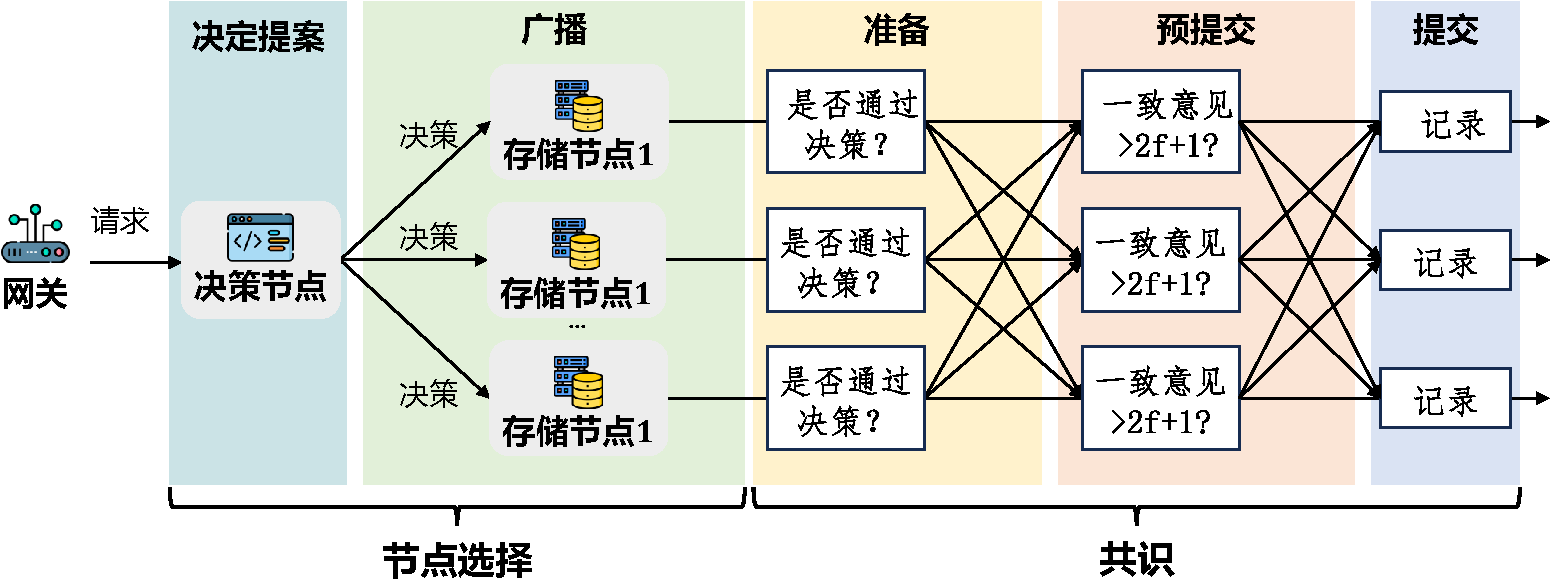
\includegraphics[width=1\linewidth]{timechain/pbft.pdf}
    \caption{中心化节点选择的工作流}
    \label{fig:pbft}
\end{figure}

如\autoref{fig:pbft}所示,中心化节点选择的流程如下:
\begin{enumerate}
    \item \textbf{决定提案}:由一个或一组节点负责评估网络中各个存储节点的信誉,根据节点的历史表现、可靠性和性能指标等因素,选择出适合承担数据存储任务的节点。
    \item \textbf{广播}:决策节点(组)将最佳存储节点的提案广播给$3f+1$个存储节点。
    \item \textbf{准备}:每个存储节点决策是否通过最佳存储节点的提案,并将决策结果广播给其他的存储节点。
    \item \textbf{预提交}:当每个节点收到大于$2f+1$个相同信息(是否通过提案)时,视作该节点与其他节点的信息充分交流,并将综合的投票结果广播给其他存储节点。
    \item \textbf{提交}:当每个节点收到$2f+1$个信息时,选择多数一致的决策记录上链。由于该网络中最多存在$f$个恶意节点,因此该阶段的决策中,虚假信息的数量一定少于诚实信息,所以该系统并不会受到恶意节点的威胁。
\end{enumerate}

在这样的节点选择流程中,中心化节点选择引入了单点故障的风险,即如果中心节点发生故障或被恶意攻击,整个系统的节点选择和数据存储过程可能会受到影响,导致服务中断或数据丢失。
同时,这种中心化的节点选择也会导致系统的扩展性受限。
随着网络节点数量的增加,中心节点需要处理的信息量也会增加,这可能导致选择过程的延迟增加,影响整个系统的响应速度。
中心节点的计算和存储能力可能成为系统的瓶颈,限制了系统处理大规模数据的能力。

而且,共识形成过程与节点选择过程完全分离会使系统的安全性会受到威胁。
这是因为,共识过程负责确保所有节点对数据状态达成一致,而节点选择过程决定了哪些节点参与到共识中。
如果这两个过程分离,恶意节点可能利用这一点来破坏系统的安全性,例如通过选择不可靠的节点参与共识过程,从而影响数据的完整性。

\section{结合共识的节点选择过程}

在前一节中,本文介绍了中心化节点选择的具体过程。
仔细观察该流程可以发现,共识过程中涉及了两次信息广播,每次信息广播都需要所有存储节点去中心化地决策。
考虑到中心化节点选择带来的风险,TimeChain创新性地将节点选择过程与共识的计算和广播过程结合,提出了一种基于共识机制的节点选择算法。

在该节点选择过程中,TimeChain利用信息广播阶段来交换各节点对存储节点的去中心化评估过程。
具体而言,TimeChain的节点选择过程包括\textbf{请求}、\textbf{准备}、\textbf{预提交}、\textbf{提交}和\textbf{回复},其详细步骤如~\autoref{fig:consensus}所示,伪代码如~\autoref{algo:consensus}所示。
与PBFT共识类似,在\textbf{请求}阶段,网关向系统中的所有节点发送请求,共识节点将在\textbf{回复}阶段将获得的结果返回给网关。
同样,类似于PBFT共识,本文假设恶意节点的数量为$f$,所有存储节点的数量超过$3f+1$。
接下来,本文将分别介绍其中的核心阶段:\textbf{准备}、\textbf{预提交}和\textbf{提交}。

\begin{figure}[t]
    \centering
    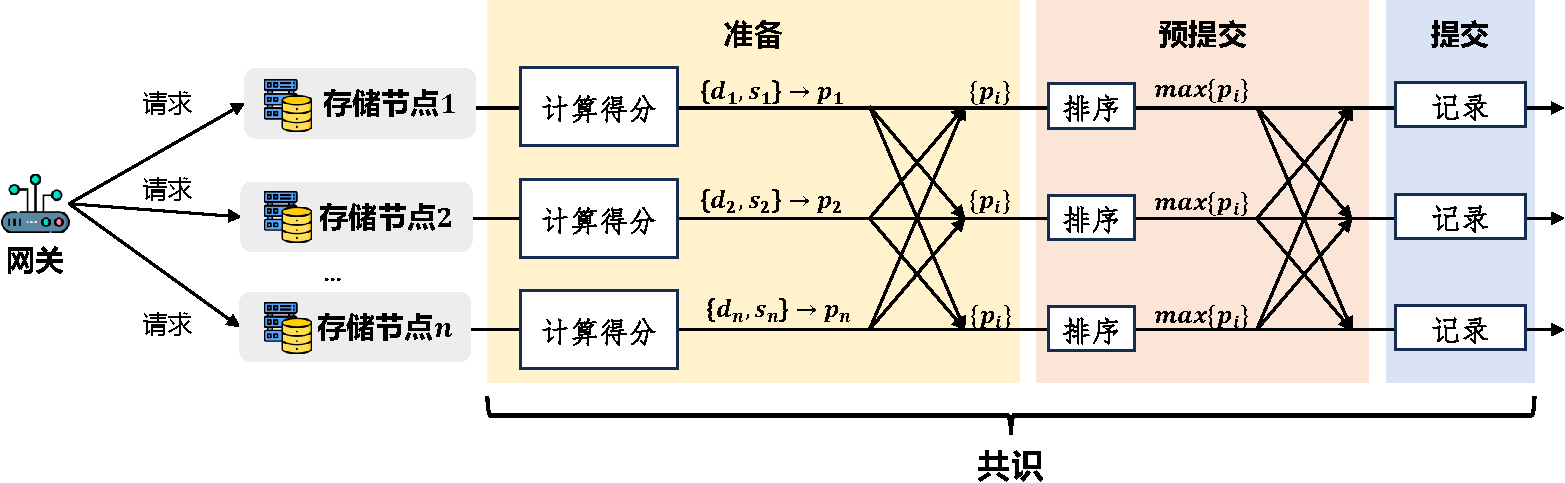
\includegraphics[width=1\linewidth]{timechain/consensus.pdf}
    \caption{基于共识的节点选择机制工作流}
    \label{fig:consensus}
\end{figure}

\begin{algorithm}
	\caption{共识过程}
	\label{algo:consensus}
	\begin{algorithmic}[1]
        \renewcommand{\algorithmicrequire}{ \textbf{准备阶段}}
        \REQUIRE
            \STATE $request \gets \textit{receive}(REQUEST)$
            \IF{$request$ 有效}
                \STATE $d_i \gets \textit{distance}(i.pos, request.pos)$ //计算节点$i$和请求节点之间的距离
                \STATE $s_i \gets i.space$ //获取节点$i$的剩余存储空间
                \STATE 通过\autoref{eq:score}计算$p_i$
                \STATE $\textit{broadcast}(p_i, \textit{PREPARE})$  //广播$p_i$
            \ENDIF

        \renewcommand{\algorithmicrequire}{ \textbf{预提交阶段}}
        \REQUIRE
            \STATE $\{p_i\} \gets \textit{receive}(p_i, \textit{PREPARE})$  //接收其他节点的\textit{PREPARE}消息
            \IF{$\textit{count}(\textit{PREPARE}) > 2 * f + 1 \textit{ 且超时}$}
                \STATE $P' \gets sort \{p_i\}$ //将$n$个节点根据信誉从高到低排序
                \STATE $P \gets \{\}$   //初始化结果集
                \FOR{$p_i \in P'$}
                    \IF{$p_i \textnormal{的计算过程可信}$}
                        \STATE \textnormal{增加$p_i$到$P$中}    //验证节点选择是否可信
                    \ENDIF
                    \IF{$count(P)>n$}
                        \STATE \textit{break}     //最佳存储节点已满足要求
                    \ENDIF
                \ENDFOR
                \STATE $\textit{broadcast}(P, \textit{PRECOMMIT})$  //广播最佳存储节点
            \ENDIF

        \renewcommand{\algorithmicrequire}{ \textbf{提交阶段}}
        \REQUIRE
            \STATE $P \gets \textit{receive}(P, \textit{PRECOMMIT})$    //接收其他节点的\textit{PRECOMMIT}消息
            \IF{$count(P) > f + 1$} 
                \STATE $\textit{commit}(P)$ //提交最佳存储节点
            \ENDIF
	\end{algorithmic}
\end{algorithm}

\subsection{准备阶段}
在该阶段,每个节点通过考虑存储节点的距离、信誉等来计算分数,并将分数广播给所有其他节点。
TimeChain选择距离、剩余存储和存储质量作为指标,原因如下:
根据图~\autoref{fig:dis_cdf},本文发现存储节点的距离会影响数据访问延迟。
因此,本文选择距离作为一个重要的指标。
此外,受到FileCoin~\cite{bauer2022filecoin}的启发,剩余存储空间和存储质量也是选择存储节点的重要因素。
剩余存储空间可以直接影响存储提供商的服务能力,而存储质量可以影响数据的完整性。
第$i$个节点的得分计算公式如下:

\begin{equation} 
    \label{eq:score}
    p_i=\alpha\cdot d_i+\beta\cdot s_i+\gamma\cdot q_i
\end{equation}

其中$d_i$表示第$i$节点和客户端节点之间的距离;$q_i$表示存储服务质量,可以从链上的服务记录中评估;$s_i$表示节点的剩余存储空间。
所有这些数据都可以在链上找到。
$\alpha$、$\beta$和$\gamma$是加权参数,这些系数可以根据特定的系统需求和性能要求进行调整。
例如,可以增加的权重以优先考虑存储完整性,而可以调整的权重以降低延迟。

\subsection{预提交阶段}
在本阶段,共识节点从其他节点接收准备好的消息集$\{p_i\}$。
当此节点的计时器超时并且收到超过$2f+1$个PREPARE消息时,共识节点根据它们收到的信誉优先级$\{p_i\}$决定最佳存储提供者。
如果每一轮共识只返回最近的节点,由于距离对信誉计算机制的影响,一些较近节点的存储压力可能会非常高。
为了平衡负载,共识节点将返回一组信誉最高的$n$节点,供网关随机选择,而不是信誉最高的节点。

为了防止恶意节点在\textbf{准备}阶段中的欺诈行为,在\textbf{预提交}阶段,共识节点的排序过程也需要对源节点的计算过程进行验证。
每个共识节点首先会对所有节点的信誉进行排序。
然后,共识节点会根据信誉由高到低的顺序,逐个验证节点的计算过程是否可信。
如果发现某个节点的计算过程不可信,共识节点将忽略该节点的信誉,继续验证下一个节点。
当共识节点收到的信誉最高的$n$个节点的信誉时,共识节点将这些节点返回给网关。

\subsection{提交阶段}
在\textbf{提交}阶段,所有节点都将收到其他节点推荐的最佳存储决策。
当相同的预提交消息的数量超过$f+1$时,此节点将向网关提交最佳存储节点集,由网关来决定最终的存储节点。
由于该网络中最多存在$f$个恶意节点,因此在\textbf{提交}阶段,虚假信息的数量一定少于诚实信息,所以该系统并不会受到恶意节点的威胁。

\section{共识过程的安全性分析}
本文在这里考虑这一共识协议的安全性。
由于TimeChain的共识协议只是基于PBFT添加了额外的信息,本文只考虑\textbf{准备}和\textbf{预提交}阶段额外信息带来的安全风险。

在\textbf{准备}阶段,如果一个节点伪造了自己的分数,网关可以很容易地检查分数的真实性,因为评估数据源都可以在链上找到。
一旦节点伪造了其信誉,该行为也将被记录在链上,从而影响下一次的信誉评估。
此外,由于最后只选择了一个存储节点,网关不关注所有节点得分的真实性,只关注所选节点的得分。

在\textbf{预提交}阶段,如果任何节点伪造了最终得分,则不会影响最终结果。
这是因为对于包含$f$拜占庭节点的$3f+1$节点的网络,必须在\textbf{提交}阶段获得相同的结果。

\section{本章小结}
在本章中,本文专注于TimeChain中存储节点选择模块。
从前面的测试中,本文认识到,存储节点与网关之间的距离直接影响数据访问延迟,而存储节点的可靠性则关乎数据的完整性和安全性。
因此,本文提出了一种基于共识协议的节点选择机制,该机制综合考虑了节点间的距离和历史服务记录,以全面评估存储节点的优劣。

本文分析了现有系统如Storj、CoopEdge和PipeEdge的局限性,指出它们依赖于集中式的节点选择服务,存在单点故障的风险。
为了解决这一问题,本文将节点选择过程与共识机制紧密结合,提出了一种新的节点选择算法。
该算法包括请求、准备、预提交、提交和回复五个阶段,通过这一流程,本文能够在确保安全性的同时,选择出最佳的存储节点。

在安全性分析中,本文证明了所提出的共识协议在PBFT基础上增加的信息并未引入额外的安全风险,因此该机制是安全的。
本文的共识协议考虑了准备阶段和预提交阶段的安全性,确保即使在存在恶意节点的情况下,系统也能正确选择出最佳的存储节点。

\chapter{基于LSH树的验证机制}
\label{sec:lsh}
从本文的测量数据中可以分析出,在传输的数据中,数据完整性证明几乎占据了一半的比例。
这些证明通常以默克尔树的形式组织,由一连串的哈希值构成。
在默克尔树结构中,非叶子节点的哈希数量与原始数据点的数量大致相同。
鉴于物联网数据单元的大小与哈希值相近,这意味着为了验证数据的完整性,需要传输的数据量几乎是原始数据量的两倍。
在数据传输过程中,如何减少完整性证明大小,成为了一个亟待解决的难题。

\section{LSH树结构与工作流程}

\begin{figure}[t]
    \centering
    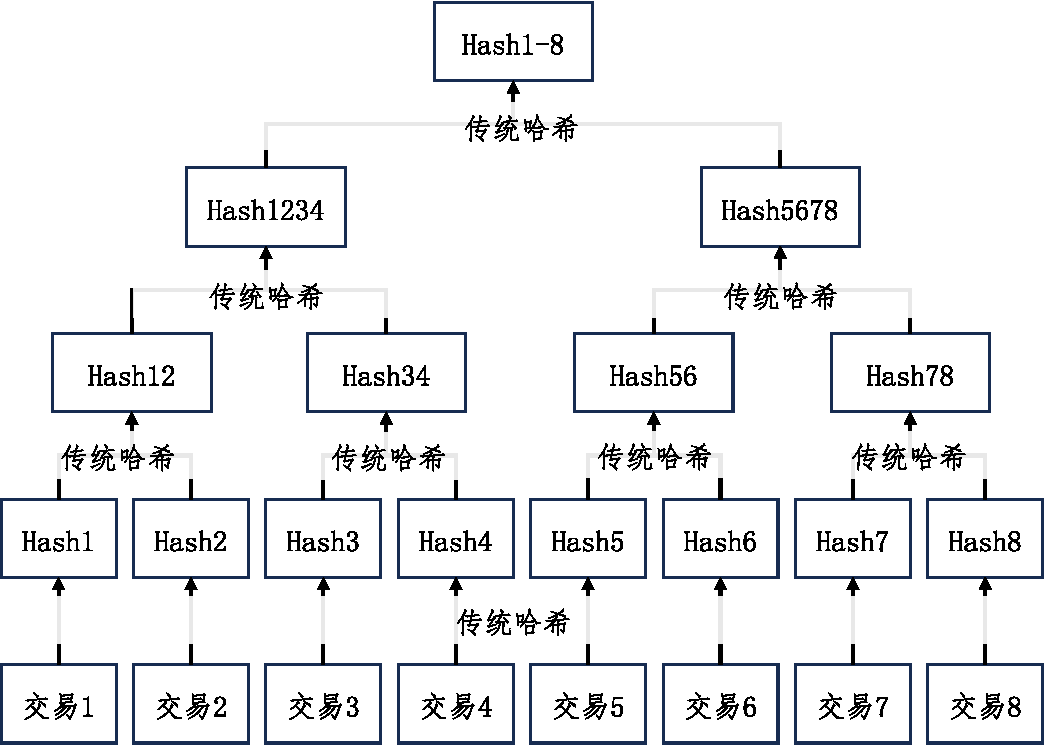
\includegraphics[width=0.8\linewidth]{timechain/merkle.pdf}
    \caption{默克尔树的结构}
    \label{fig:merkle}
\end{figure}

默克尔树(Merkle Tree)作为一种轻量级的完整性验证机制,在许多区块链平台中广泛使用。
如~\autoref{fig:merkle}所示,默克尔树是一种二叉树结构,其中每个非叶节点都是其两个子节点的哈希值。
具体来说,叶节点通常包含底层交易的哈希值,而非叶节点则包含其左右子节点哈希值的组合哈希。
树的根节点最终形成一个单一的哈希值,称为默克尔根(Merkle Root),这个哈希值将被存储在链上。
通过这种方式,默克尔树能够将大量数据压缩成一个固定长度的哈希值,并允许高效地验证任何单个数据项是否属于该集合。

为了给出完整性证明,给定一个数据项,可以通过提供一条“默克尔路径”来证明该数据项属于某个默克尔树。
这条路径包括从叶节点到根节点所需的所有兄弟节点哈希值,使得验证者能够在不获取整个数据集的情况下确认成员资格。
例如,要证明交易8的有效性,数据存储方可以提供$Hash7, Hash56, Hash1234$。
如果最终发现$hash(hash(hash(hash($交易8$),Hash7),Hash56),Hash1234)$与记录在链上的$Hash1-8$相符,则说明交易8确实在该交易集合中。

在大量数据存储的场景中,为了尽量减少重构默克尔树的计算开销,使数据存储方可以对用户的请求做出快速响应,这个默克尔树的非叶子节点也需要被存储在存储节点。
然而,默克尔树的节点数量大,节点数据较长。
如~\autoref{fig:merkle}所示,对于8个交易,默克尔树需要生成15个非叶子节点的哈希值。
由于物联网元数据较小,与哈希值长度基本相当,因此默克尔树的完整性证明较大,在验证阶段需要占据大量带宽,在存储方也会占用较多存储空间。

\begin{figure}[t]
    \centering
	\begin{minipage}{0.6\linewidth}
        \centering
        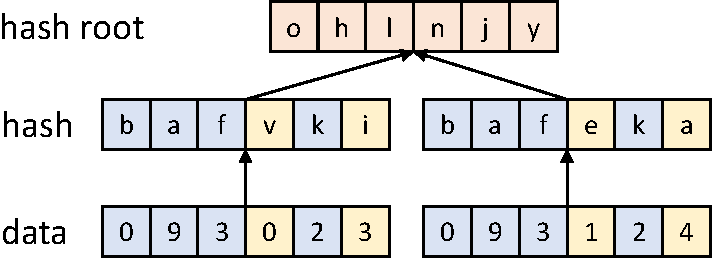
\includegraphics[width=1\linewidth]{timechain/lsh-tree.pdf}
        \caption{LSH树结构}
        \label{fig:lsh_tree}
	\end{minipage}
\end{figure}

深入分析物联网数据的特性后,本文注意到物联网数据的变化通常较为缓慢,短期内不太可能发生剧烈变动。
针对这些高度相似的数据点,LSH算法能够从相似的原始数据中产生相似的哈希结果。
LSH算法的这一特性保证了即使在哈希处理之后,相似的物联网数据点仍然保持相似性。
基于这一观察,本文设计了一种创新的基于LSH树的验证机制,它采用LSH算法替代了传统默克尔树中使用的通用哈希函数。
通过仅传输LSH哈希值的差异部分,本文能够显著减少在验证过程中需要传输的数据量,从而提高了数据传输的效率。

本文在~\autoref{fig:lsh_tree}中展示了LSH树的一个例子。
具体来说,对于批处理中的数据,本文采取类似于默克尔树的步骤,首先对原始数据执行局部敏感哈希。
对于哈希结果,本文将两个相近的哈希合并为一个字符串,并计算该字符串的局部敏感哈希值。
然后,本文逐层向上重复这个过程,直到本文得到一个唯一的哈希值,即哈希根。
在第一级哈希中,由于原始数据的高度相似性,哈希值的许多位是相同的。
因此,在传输第一级哈希值时,本文只能传输不同的比特以减少传输延迟。
同样,由于第一级哈希中存在局部相似性,第二级哈希中的许多比特也将相似。
通过类比,对于每一层的哈希值,本文只需要传输哈希差比特,从而进一步减少了传输的数据量。

\section{LSH树的尾部合并机制}

\begin{figure}[t]
    \centering
	\begin{minipage}{0.8\linewidth}
        \centering
        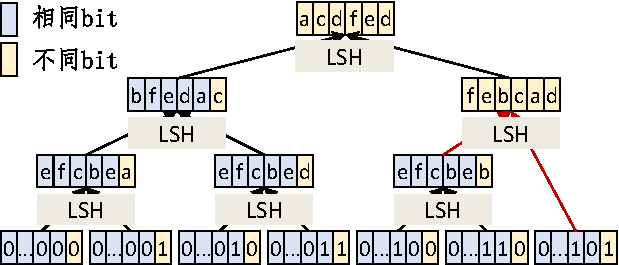
\includegraphics[width=1\textwidth]{timechain/tail_merging_lsh.pdf}
        \caption{非满二叉LSH树}
        \label{fig:tail_merging_lsh}
	\end{minipage}
\end{figure}

\begin{figure}[t]
    \centering
	\begin{minipage}{0.8\linewidth}
        \centering
        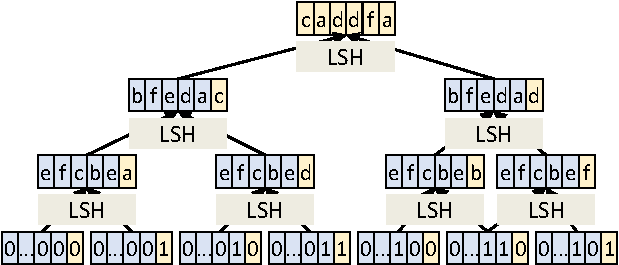
\includegraphics[width=1\textwidth]{timechain/tail_merging_tail.pdf}
	\end{minipage}
	\caption{尾部合并下的非满二叉LSH树}
	\label{fig:tail_merging_tail}
\end{figure}

在一个完整的二叉树中,LSH树可以通过成对地批量合并数据来执行局部敏感哈希。
然而,如果批处理中的数据数量不足以形成完整的二叉树,那么像默克尔树一样构建哈希树将导致相似性的丧失。
例如,在~\autoref{fig:tail_merging_lsh}中,一批中有7个数据点,对于一个完整的二叉树来说,这个大小是不满足的。
在第一轮哈希中,前6个数据成对执行LSH。
由于原始数据的相似性,这6个数据的哈希结果是相似的。
在第二轮哈希中,由于数据5-6和第7个原始数据的第一轮哈希结果非常不同,这两个数据的哈希结果也与数据点1-4的哈希结果非常不一样。
在执行完整性证明时,需要传输所有这些不同的哈希数据位,这增加了传输的数据量。

为了解决这个问题,本文引入了尾部合并策略,将非全二叉树的尾部节点与同一层的前节点合并。
如~\autoref{fig:tail_merging_tail}所示,在第一轮哈希中,本文将第7个节点和第6个节点合并,以尽可能保持数据的相似性。
数据6-7的哈希结果是\texttt{efcbeb},数据5-6的哈希值是\texttt{efcbef}。
显然,在第一轮哈希中存在很高的相似性,并且可以保持到下一级哈希。
这将传输的哈希值大小从12位减少到7位,代价是在第一轮哈希中只传输了1个不同的比特。
这样,在进行完整性证明时,本文只需要传输不同的哈希位,从而减少了传输的数据量。

\section{LSH树的安全性分析}
鉴于本文提出的解决方案中采用了LSH树替代了传统的默克尔树,对LSH树的安全性进行深入分析变得至关重要。
LSH树的设计初衷是为了减少数据传输量,同时保持数据验证的准确性。
然而,这种替代可能会引入新的安全风险。
本文主要关注数据篡改问题,即在LSH树结构中,存储提供者是否能够通过改变数据内容来得到与未篡改数据相同的哈希值。
为了评估这一风险,本文对LSH树的不同层级进行了广泛的测试,以确定在何种程度上篡改数据而不被检测到是可行的。

测试结果表明,在最接近数据源的哈希层,也就是LSH树的最底层,哈希值的平均差位数达到了170位。
这一数值远超过了广泛使用的MD5和SHA1哈希算法的安全性标准,这些标准现在在物联网场景中非常常用~\cite{chi2017hashing,landge2018secured}。
因此,LSH树在底层提供的170位的哈希差位数,为数据完整性提供了更强的安全保障。

对于LSH树靠近根节点的高层级,虽然哈希差位数较少,但这并不意味着篡改数据变得容易。
实际上,由于LSH树的结构特性,即使是高层级的少量哈希差异也足以被检测出来,因为这些差异会随着树的结构向上传播,最终影响到根哈希值。
因此,任何对原始数据的篡改,无论在树的哪一层,都很难不被察觉。

综上所述,LSH树不仅提供了与传统默克尔树相似的数据验证功能,而且在安全性方面仍然符合物联网场景的需要。

\section{本章小结}
在本章中,本文针对物联网数据完整性验证过程中的数据传输延迟问题,提出了一种基于LSH树的新型验证机制。
本文发现,在传输的数据中,数据完整性证明占据了相当大的比例,且通常以默克尔树的形式组织,这导致为了验证数据完整性需要传输的数据量几乎是原始数据量的两倍。
为了解决这一问题,本文利用物联网数据变化缓慢且高度相似的特性,采用LSH算法替代了传统默克尔树中的通用哈希函数,通过仅传输LSH哈希值的差异部分,显著减少了验证过程中需要传输的数据量。

本文详细分析了LSH树的结构和工作流程,并针对非满二叉树的情况,引入了尾部合并策略以保持数据的相似性,进一步减少了传输的数据量。
此外,本文还对LSH树的安全性进行了分析,确保了其在最接近数据源的哈希层中具有足够的安全性,超过了现有的MD5和SHA1标准,在物联网场景中足够安全。

\chapter{实验结果与分析}
在本章中,本文将对TimeChain系统进行全面的实验评估,从存储延迟和查询延迟两个关键维度来验证TimeChain设计的有效性。
本文将分析TimeChain在不同查询负载和存储网络条件下的性能表现,并针对系统中的自适应聚合机制、基于共识的节点选择机制和基于LSH树的验证机制进行消融实验,以展示这些技术点对系统性能的具体提升。
通过这些实验,本文旨在展示TimeChain相比于现有解决方案在区块链存储系统中的性能优势。

\section{实验设置}
本文基于一些开源项目(如Hyperledger Fabric和IPFS)实现TimeChain。
本文使用阿里云的50台虚拟机构建了一个基于Hyperledger Fabric的底层区块链系统,每个节点配备2核CPU和4GB内存。
块大小设置为1500个交易,块间隔为1秒。
本文基于一个真实世界的存储网络~\cite{corneo2021surrounded},模拟了分布在世界各地的320个云服务器节点,并基于该集群进行了实验。
每个存储节点配置2核CPU和4GB内存,每个存储节点的存储空间为512GB。
存储节点和网关之间的距离从800公里到6000公里不等,平均为4000公里。
本文使用现有的线性回归模型~\cite{ziviani2005improving}模拟存储节点和网关之间的传输延迟。
考虑到一些存储提供商存在欺诈行为,部分远程存储的数据将有概率无法被访问到,概率为60\%。
本文使用电脑(Personal Computer,PC)作为物联网传感器的网关节点,它配备了Intel(R)Core i7-13700K CPU@5.4GHz、32GB DRAM,并运行Ubuntu 22.04。
默认聚合存储单元大小和查询大小设置为20。

\subsection{基线}
\textbf{SEBDB}~\cite{zhu2019sebdb}是链上存储的典型代表。
它通过将所有数据存储在区块链上,并使用B+树创建时间戳和设备名称的快速索引实现了对链上区块的高效访问。
在数据验证方面,SEBDB使用传统的默克尔树进行数据验证。
默克尔树通过计算数据块的哈希值,并将这些哈希值逐层组织成树结构,来实现数据完整性验证。
尽管SEBDB不是专门为物联网数据设计的链下存储解决方案,但是因为它的数据验证机制类似于TimeChain,本文将它作为对比方案。
为了保证实验的公平性,本文调整了SEBDB来记录单个数据项的存储位置并将其上传到链中,并随机选择存储节点。
这些修改确保了实验的公平性,同时更好地反映了物联网数据的特点和需求。

\textbf{FileDES}~\cite{xu2024filedes}是一个基于文件的链下存储系统。
它通过在远程节点上存储文件并在链上记录文件的哈希值来实现文件的安全存储和可靠性。
当客户端需要搜索文件时,FileDES会遍历区块链上的所有块,以获取文件的存储位置。
在数据验证方面,FileDES也使用与SEBDB相同的默克尔树。
由于FileDES是为文件存储设计的,为了确保实验的公平性,本文将FileDES改造成为适用于物联网数据的链下存储系统。
对于到达网关的物联网数据,FileDES将这些数据以固定大小、按照到达网关的顺序进行打包,并将这些数据上传到远程存储节点。

\subsection{数据集和工作负载}

本文使用了以下三个数据集进行实验:

\textbf{港珠澳大桥(Bridge)}~\cite{zhang2023edge}:
Bridge数据集包含4M条数据记录,这些数据是在5天内从港珠澳大桥上的6种传感器采集的。
这6种传感器与桥梁健康监测有关,包括桥梁各个位置的振动加速度、挠度等,共计53个。
由于数据生成频率为10Hz,本文将平均数据查询范围设置为40。

\textbf{RT-IFTTT(RT)}~\cite{heo2017rt}:
RT数据集包含680K条数据记录。
这些数据是在10天内从10个真实传感器采集的值,包括温度、湿度、可见光和其他传感器。
数据以秒为单位收集,因此查询的平均范围设置为20。

\textbf{天气 (WX)}~\footnote{https://www.kaggle.com/selfishgene/historical-hourly-weather-data/}:
WX数据集包含1.5M条数据记录,其中包括来自五年内30多个城市的各种天气属性每小时测量的数据。
鉴于数据收集频率相对较低,间隔最多一小时,本文假设查询范围为10。

考虑到时间序列存储系统的存储特性~\cite{naqvi2017time},本文将这些数据集的格式转换为\\ $<measurement, field~name, field~value, timetamp>$。
$measurement$ 类似于数据表,用于组织数据,例如“天气”;
$field~name$ 用于标识不同的字段,例如“温度”;
$field~value$存储的是实际数据,比如温度传感器的实际值;
$timestamp$是时间戳,记录了数据的时间信息。
考虑到数据集的特点,本文将这些数据的大小分别固定为8B、32B、8B、8B。
因此,一条数据总共占用的存储空间为56B。

\section{总体性能评估}

\subsection{存储延迟}
\begin{figure*}[t]
    \centering
	\begin{minipage}{0.48\linewidth}
        \centering
        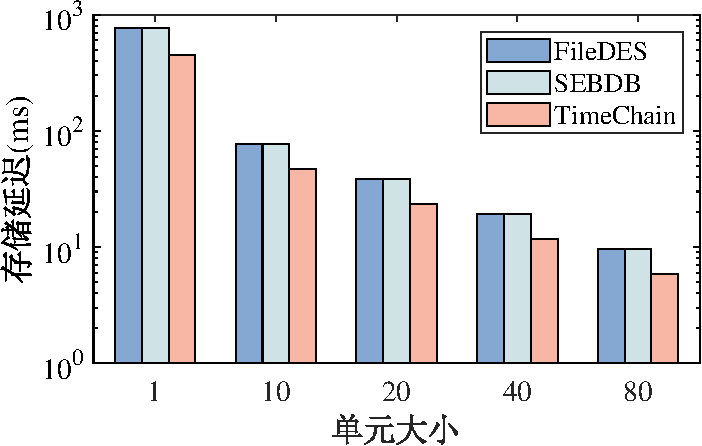
\includegraphics[width=1\textwidth]{timechain/storage_rt_eval.pdf}
        \caption{存储延迟}
        \label{fig:storage_rt_eval}
    \end{minipage}
    \quad
    \begin{minipage}{0.48\linewidth}
        \centering
        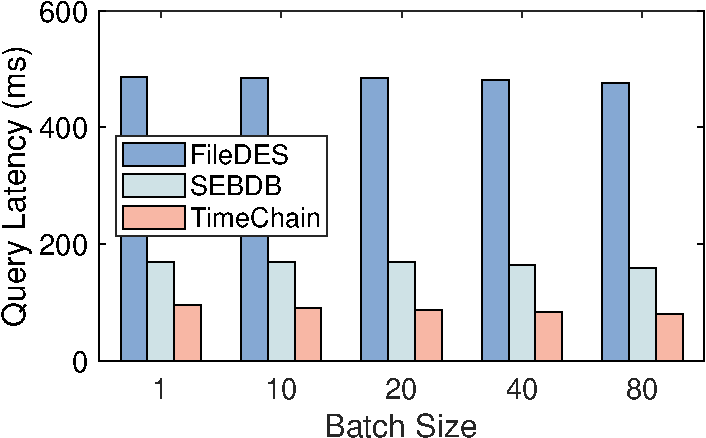
\includegraphics[width=1\textwidth]{timechain/query_rt_eval.pdf}
        \caption{查询延迟}
        \label{fig:query_rt_eval}
	\end{minipage}
\end{figure*}
本文比较了不同聚合单元大小下的存储延迟。
由于物联网设备数量众多,数据生成速度快,本文将存储延迟定义为存储10000个数据的总延迟,而不是关注单个数据的细微延迟。
如~\autoref{fig:storage_rt_eval}所示,对于不同的聚合单元大小,TimeChain的存储延迟低于SEBDB和FileDES。
这是因为TimeChain的独特打包机制和节点选择机制减少了数据传输延迟。

此外,随着聚合单元大小变大,存储延迟变小。
这是因为,对于相同数量的数据,当聚合单元较大时,数据在链中打包和记录的次数会减少。
然而,较大的聚合单元可能会引入较大的存储等待延迟。
因为一个聚合单元可能需要等待较长时间才可以被填满,才能被打包和记录。
具体的聚合单元大小需要根据实际数据产生速度和用户的需求来确定。
用户可以通过调整网关的聚合单元大小来控制实际的存储延迟。

\subsection{查询延迟}
本文比较了不同聚合单元大小的查询延迟,如~\autoref{fig:query_rt_eval}所示。
查询延迟是指基于固定查询范围随机查询数据集的平均延迟,查询范围设置为20。
从~\autoref{fig:query_rt_eval}可以看出,TimeChain的查询延迟低于其他两种方案。
这是由于TimeChain减少了数据传输延迟,原因将在~\autoref{fig:query_breakdown}中解释。

本文还可以发现,当聚合单元大小增加时,查询延迟会减少。
这是因为当聚合单元大小增加时,同一查询中涉及的聚合单元数量会减少,用户的查询结果将大概率集中在一个存储节点上。
然而,聚合单元越大,TimeChain相对于其他解决方案的改进将随着聚合单元的增大而减少。
这是因为当聚合单元非常大时,相当于将所有数据存储在一个聚合单元中。
在这种情况下,对于数据进行谱聚类切分不会导致性能提高,反而会导致对多种范围查询的灵活性降低。
此外,当大量数据集中在存储节点中时,存储系统的可扩展性和可靠性也会受到损害。

\begin{figure*}[t]
    \centering
    \begin{minipage}{0.48\linewidth}
        \centering
        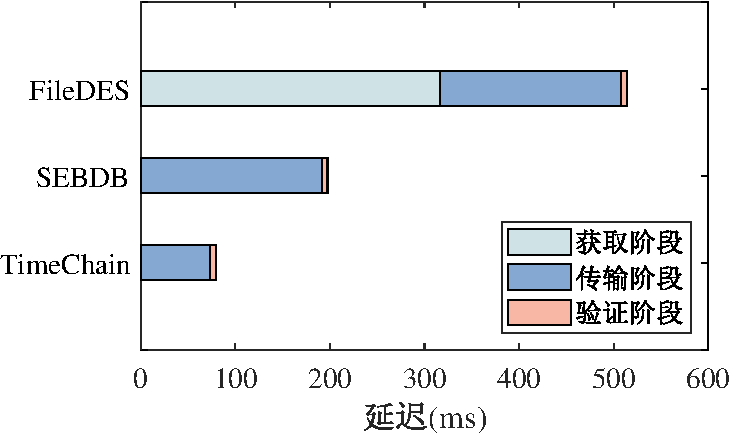
\includegraphics[width=1\linewidth]{timechain/query_breakdown.pdf}
        \caption{查询延迟分解}
        \label{fig:query_breakdown}
	\end{minipage}
	\quad
	\begin{minipage}{0.48\linewidth}
        \centering
        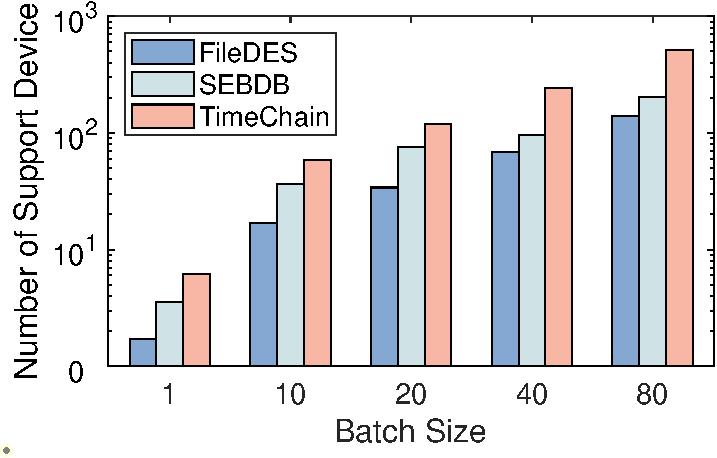
\includegraphics[width=1\linewidth]{timechain/support_device.pdf}
        \caption{最大支持存储设备数}
        \label{fig:support_device}
    \end{minipage}
\end{figure*}

\subsection{查询延迟分解}
本文进一步分析了查询延迟的细分,以确定影响整体查询性能的主要因素,如~\autoref{fig:query_breakdown}所示。
查询的延迟主要由4个阶段组成,检索、传输、验证和返回。
考虑到传感器通常选择更近的网关,返回阶段的延迟几乎可以忽略不计。
在验证阶段,三种方案的延迟相对接近,小于1ms,也可以被忽略。

在传输和检索阶段,本文发现延迟占据了查询延迟的主要部分。
特别是TimeChain的传输延迟明显低于FileDES和SEBDB。
这一优势归功于TimeChain的节点打包机制,该机制优化了数据的组织方式,减少了从存储节点获取数据的次数。
同时,TimeChain的节点选择机制通过选择地理位置更近的存储提供商进一步缩短了数据传输的距离,从而降低了传输延迟。

在检索阶段,FileDES由于需要遍历区块链上的所有块来检索数据,导致了较高的检索延迟。
这种机制在面对大量数据时效率较低,尤其是在数据量迅速增长的场景下。
相比之下,SEBDB和TimeChain通过使用B+树和R树索引结构,显著提高了检索效率,降低了延迟。
这两种索引结构允许系统快速定位到存储数据的位置,从而加快了检索速度。

\subsection{支持的最大存储设备数量}
在本小节中,本文使用的支持设备最大数量指标,即存储系统每秒可以提供存储服务的设备数量。
本文假设网关可以同时处理来自多个物联网设备的数据存储请求,并忽略网关本身的处理延迟。
所有物联网设备同时以1Hz的频率生成数据,并要求在生成下一个数据之前必须存储这些数据。
在这样的限制下,存储系统可以并行支持的最多设备数量即为支持的最大存储设备数量。
如~\autoref{fig:support_device}所示,TimeChain支持最大设备数量分别是SEBDB和FileDES的1.63倍和3.55倍。
这主要是由于TimeChain对数据传输延迟采取的优化技术,较小的数据传输延迟允许TimeChain以更快的速度存储数据。
此外,对于所有测试的方案而言,随着聚合单元大小的增加,支持的最大设备数量也随之增加。
这是因为较大的聚合单元意味着单个链上哈希可以代表更多的数据量,从而提高了单个存储单元的效率,使得系统能够支持更多的物联网设备。
特别地,当聚合单元大小达到80时,TimeChain支持的最大设备数已经达到了千级,这一结果充分展示了TimeChain在大规模物联网环境中的扩展能力和高效性。
这一性能优势不仅证明了TimeChain在处理大规模数据时的可靠性,也为未来物联网应用的发展提供了强有力的技术支持。

\begin{figure}[t]
    \centering
	\begin{minipage}{0.45\linewidth}
        \centering
        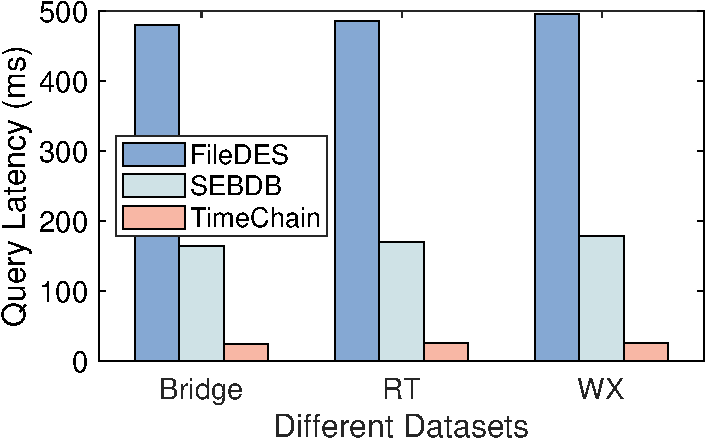
\includegraphics[width=1\textwidth]{timechain/query_diff_dataset.pdf}
        \caption{不同查询大小下的查询延迟}
        \label{fig:query_diff_dataset}
	\end{minipage}
	\quad
	\begin{minipage}{0.45\linewidth}
        \centering
        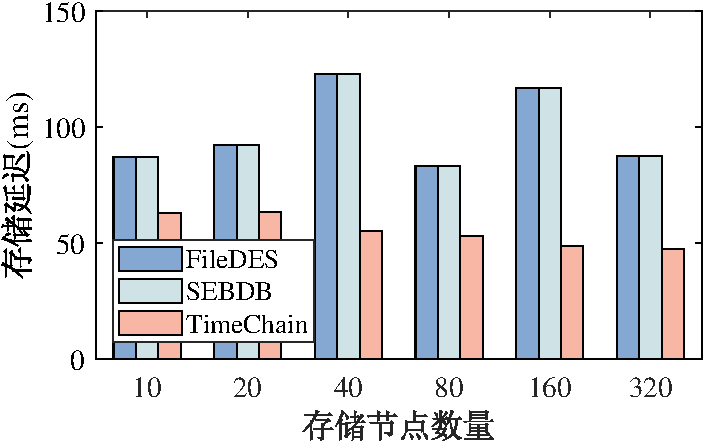
\includegraphics[width=1\textwidth]{timechain/storage_diff_storage_nodes.pdf}
        \caption{不同存储网络下的存储延迟}
        \label{fig:storage_diff_storage_nodes}
    \end{minipage}
\end{figure}

\section{性能影响因素评估}
\subsection{不同查询大小下的查询延迟}
本文比较了三种不同查询大小数据集(Bridge、RT和WX)的查询性能,结果如~\autoref{fig:query_diff_dataset}所示。
三个数据集中工作负载的平均查询大小分别为40、20和10。
本文可以发现,这三种解决方案的查询延迟通常随着查询大小的增加而增加,即WX最小,RT次之,Bridge最大。
这是因为更大的查询大小涉及了更多的聚合单元,因此可能需要去更多的存储节点获取数据,从而增加了数据传输延迟。
本文观察到,与SEBDB和FileDES相比,当查询大小变大时,TimeChain的聚类算法带来的性能改进也会增加。
这是因为当查询大小变大时,SEBDB和FileDES通常需要从比TimeChain更多的节点获取数据,而TimeChain可以通过聚类算法减少数据获取的次数,从而减少数据传输延迟。

\subsection{不同存储网络规模下的存储延迟}
本文比较了不同存储网络规模下每种解决方案的存储延迟,如~\autoref{fig:storage_diff_storage_nodes}所示。
随着存储节点数量的增加,TimeChain的存储延迟呈下降趋势。
这一现象的原因在于,TimeChain的网关在选择存储提供商时拥有更大的灵活性,能够从更多的节点中选择,从而增加了选择到地理位置更接近的存储节点的机会,这自然降低了数据传输的时间。
相比之下,FileDES和SEBDB由于采用了随机选择存储节点的机制,它们在存储节点数量增加时,并没有表现出存储延迟的显著变化。
这种随机性导致了这两种方案在存储延迟上缺乏可预测性,且在不同存储网络规模下,它们的性能波动较大。
由于FileDES和SEBDB在选择存储节点时没有考虑节点的具体位置信息,因此它们无法充分利用增加的节点来优化存储延迟。
这就导致了即使在存储节点数量增加的情况下,这两种方案的存储延迟仍然保持在一个相对较高的水平,且波动较大,这在一定程度上限制了它们在大规模存储网络中的应用潜力。

\section{消融实验}
\subsection{聚类算法}
\begin{figure*}[t]
    \centering
	\begin{minipage}{0.96\linewidth}
        \subfloat[查询延迟]{
            \centering
            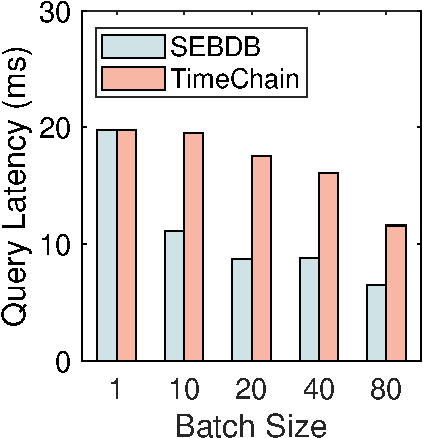
\includegraphics[width=0.45\textwidth]{timechain/ratiocut_latency_eval.pdf}
            \label{fig:ratiocut_latency_eval}
        }
        \subfloat[跨越的batch]{
            \centering
            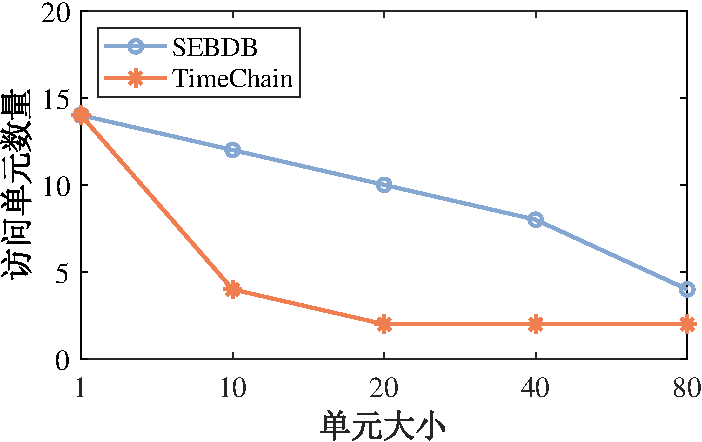
\includegraphics[width=0.47\textwidth]{timechain/ratiocut_batch_eval.pdf}
            \label{fig:ratiocut_batch_eval}
        }
        \caption{聚类算法消融实验} 
    \end{minipage}
\end{figure*}

本文比较了聚类算法的效果,并将TimeChain与SEBDB进行了比较。
如图~\autoref{fig:ratiocut_latency_eval}所示,与SEBDB相比,TimeChain的网络传输延迟减少了40.3\%。
这是因为SEBDB的打包节点未能充分考虑用户查询的规律性,只是将物联网数据根据到达网关的顺序进行打包。
这导致在处理数据拥有者请求的数据时,SEBDB不得不访问多个存储提供商所管理的聚合单元,增加了数据检索的复杂性和延迟。
相比之下,TimeChain采用了谱聚类算法,这种算法能够根据用户请求的特征对来自特定传感器的数据进行打包。
这种方法不仅优化了数据在存储节点中的分布,还减少了数据访问时需要跨越的聚合单元数量。
如图~\autoref{fig:ratiocut_batch_eval}所示,TimeChain访问的聚合单元数量比SEBDB少了59.3\%,这表明TimeChain在减少数据访问延迟和提高查询效率方面具有明显优势。

\begin{figure*}[t]
    \centering
    \begin{minipage}{0.96\linewidth}
        \vspace{0.5ex}
        \subfloat[查询延迟]{
            \centering
            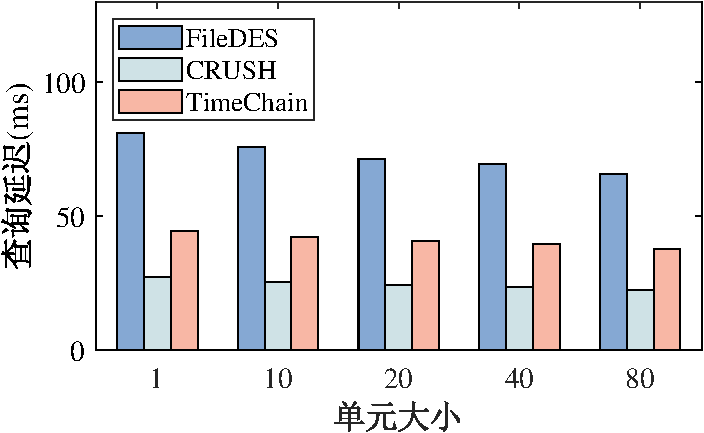
\includegraphics[width=0.45\textwidth]{timechain/consensus_latency_eval.pdf}
            \label{fig:consensus_latency_eval}
        }
        \subfloat[存储服务质量]{
            \centering
            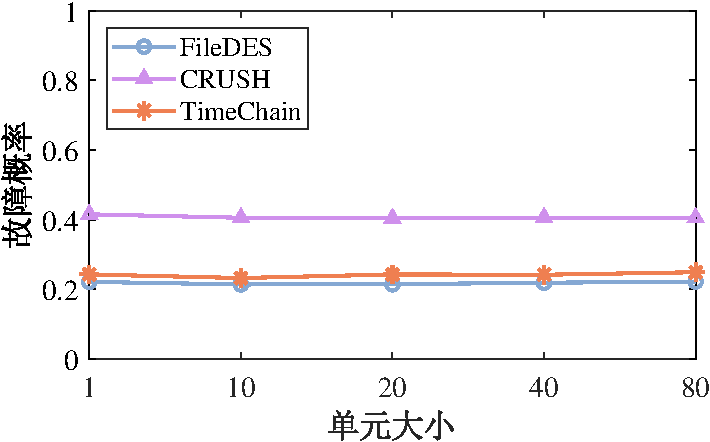
\includegraphics[width=0.47\textwidth]{timechain/consensus_prob_eval.pdf}
            \label{fig:consensus_prob_eval}
        }
        \caption{节点选择消融实验} 
    \end{minipage}
\end{figure*}

\subsection{节点选择}
本文在图~\autoref{fig:consensus_latency_eval}和图~\autoref{fig:consensus_prob_eval}中显示了TimeChain、FileDES~\cite{xu2024filedes}和CRUSH~\cite{weil2006ceph}在节点选择方面的性能差异。

FileDES通过基于节点信誉的筛选机制,确定了一组受信任的存储节点,并在此基础上随机选择节点进行数据存储。
这种方法的优点在于提高了数据存储的安全性,因为只有信誉良好的节点才被考虑用于存储。
然而,由于缺乏对节点地理位置的考虑,FileDES的随机选择可能导致选择了距离较远的节点,从而增加了数据传输的延迟,影响了整体性能。

CRUSH则采取了一种基于物理位置的策略,优先选择距离最近的节点进行数据存储。
这种策略在不考虑节点故障和可靠性的情况下,能够显著减少数据传输的时间。
然而,CRUSH方案的一个主要缺陷是它没有充分考虑节点的可靠性,如图~\autoref{fig:consensus_prob_eval}所示,这导致有41\%的节点可能无法提供有效的存储服务,这对于需要高可靠性的存储系统来说是一个严重的缺陷。

与FileDES和CRUSH相比,TimeChain在节点选择上采取了一种综合考虑节点物理距离和信誉的策略。
TimeChain不仅考虑了节点的地理位置以减少传输延迟,还考虑了节点的历史服务记录和信誉,以确保所选节点的可靠性。
这种综合考虑的方法使得TimeChain在响应时间和服务概率方面都展现出了最佳性能。
尽管TimeChain选择的节点可能不是物理距离上最近的,但通过平衡节点的距离和服务质量,TimeChain能够提供更稳定和高效的存储服务。

\begin{figure*}[t]
    \centering
    \begin{minipage}{0.96\linewidth}
        \vspace{-0.5ex}
        \subfloat[查询延迟]{
            \centering
            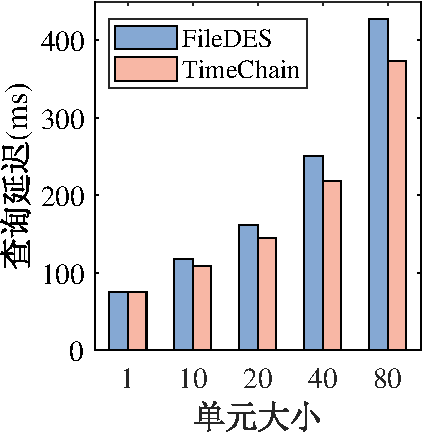
\includegraphics[width=0.45\textwidth]{timechain/lsh_latency_eval.pdf}
            \label{fig:lsh_latency_eval}
        }
        \subfloat[完整性证明大小]{
            \centering
            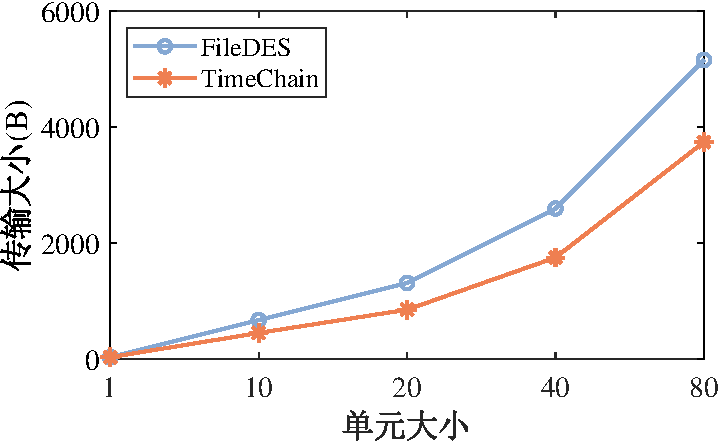
\includegraphics[width=0.47\textwidth]{timechain/lsh_size_eval.pdf}
            \label{fig:lsh_size_eval}
        }
        \caption{LSH树消融实验} 
    \end{minipage}
\end{figure*}

\subsection{LSH树}
本文比较了FileDES和TimeChain的网络传输延迟,如图~\autoref{fig:lsh_latency_eval}所示。
与FileDES相比,TimeChain的数据传输延迟减少了10.9\%。
这主要是来源于TimeChain对数据传输量的优化。
在物联网中,局域网内传感器设备的数量众多,且这些设备通常以高频率持续生成数据。
如图~\autoref{fig:lsh_size_eval}所示,由于TimeChain使用LSH作为哈希算法,通过网络传输的数据量大大减少。
这种数据量的减少不仅降低了存储和查询操作的延迟,还显著减轻了存储提供商的存储负担。
对于存储提供商而言,这意味着更低的存储成本和更高的数据处理效率。
同时,对于整个存储系统来说,减少了数据传输量还有助于提高系统的吞吐量和响应速度,尤其是在高负载或资源受限的环境中。

\section{本章小结}
在本章中,本文对TimeChain系统进行了全面的实验评估,以验证其在存储性能方面的优势。
通过在模拟的全球存储网络上进行测试,本文比较了TimeChain与现有解决方案,SEBDB和FileDES,在存储延迟和查询延迟方面的表现。
实验结果表明,TimeChain在减少查询延迟和存储延迟方面具有显著优势,平均查询延迟降低了64.6\%,存储延迟降低了35.3\%。

本文还分析了不同查询负载和存储网络规模对TimeChain性能的影响,发现随着聚合单元大小的增加,TimeChain的存储和查询性能得到了进一步的提升。
此外,TimeChain在支持最大存储设备数量方面也展现出了其可扩展性,与SEBDB和FileDES相比,分别增加了1.63倍和3.55倍。

为了进一步验证TimeChain设计中关键技术点的有效性,本文进行了消融实验。
实验结果证实了自适应聚合机制、基于共识的节点选择机制和基于LSH树的验证机制在提升系统性能方面的重要作用。
特别是LSH树机制,通过减少传输的数据量,显著降低了网络传输延迟。

\chapter{总结与展望}

\section{总结研究}
本文提出了TimeChain,一个基于区块链的物联网时序数据高效可信存储系统。
针对物联网场景下数据生成速度快、数据量大、需要高效率和高可信度的数据存储问题,TimeChain仅将每批数据的哈希值存储在链上,而完整的原始数据则保存在链外。
TimeChain针对范围查询性能的瓶颈,分别提出了自适应聚合机制、基于共识的存储节点选择机制和基于LSH树的数据完整性验证机制。
本文的主要创新点总结如下:

1. 提出了一种面向物联网数据的基本处理方案,即把每批数据的哈希值存储在链上以减少数据开销并提高存储效率。
本文也对这个基本方案进行了一系列测量,发现了基本方案性能较差的核心原因,为后续的优化提供了方向。

2. 设计了一种自适应聚合机制,通过构建基于历史查询的无向加权图,将数据打包问题转化为图划分问题,并使用谱聚类算法优化数据的批处理存储,以减少聚合查询期间的节点访问次数。

3. 提出了一种基于共识的存储节点选择机制,结合存储节点信誉和传输距离,通过将共识过程与节点选择相结合,以减少传播延迟并提高节点选择的安全性。

4. 创新性地设计了基于LSH树的数据完整性验证机制,利用物联网数据的局部相似性,仅传输证明的非冗余部分,显著减少了完整性验证所需的数据量。

本文基于开源组件实现了TimeChain系统,并在一个模拟的存储网络中进行评估。
实验结果表明,TimeChain相比于现有的基于区块链的存储系统,平均减少了64.6\%的查询延迟和35.3\%的存储延迟,证明了其在存储性能方面的显著优势。

\section{未来工作}
在未来的工作中,本文计划针对TimeChain系统进行以下几方面的研究和改进,以进一步提升系统性能并适应不同的应用场景。

1. 本文将在真实的环境中实现并部署TimeChain,以验证其在实际应用中的性能和可靠性,确保在实际部署中能够满足各种应用场景的需求。
这包括在不同的网络条件下,对算法的响应时间和吞吐量进行评估。

2. 由于PBFT算法存在吞吐量有限的问题,对于数据生成速度逐渐增加和设备逐渐扩张的物联网场景,PBFT可能无法满足系统的性能需求。
本文计划探索其他轻量化或异步共识算法,如Raft和Tendermint,将这些高效算法与TimeChain结合。
这些算法能够在不牺牲安全性的前提下,减少通信开销,提高TimeChain的响应速度和吞吐量,特别适合资源受限的物联网设备。
本文也将考虑其他提升区块链性能的方法,如分片、侧链等,以提高系统的可扩展性和性能,并进一步分析可能带来的安全风险。

3. 在引入新的共识算法的同时,本文也将重点关注TimeChain的安全性和稳定性。
这包括对本文所提共识协议和LSH树的安全性进行实验验证。
本文将在一个真实、存在欺诈节点的物联网环境中进行实验,分析TimeChain对恶意网络的容忍性,以及对数据完整性和隐私性的保护能力。
